\documentclass[11pt,a4paper]{article}

\usepackage[T1]{fontenc}
\usepackage[utf8]{inputenc}
\usepackage[french]{babel}
\usepackage{lmodern}
\usepackage{microtype}
\usepackage{geometry}
\geometry{margin=2.2cm}
\usepackage{graphicx}
\usepackage{booktabs}
\usepackage{array}
\usepackage{tabularx}
\usepackage{subcaption}
\usepackage{xcolor}
\usepackage{enumitem}
\usepackage{hyperref}
\hypersetup{
  colorlinks=true,
  linkcolor=black,
  urlcolor=blue
}
\setlength{\parindent}{0pt}
\setlength{\parskip}{0.45em}
\setlist[itemize]{leftmargin=*, itemsep=0.25em, topsep=0.25em}
\renewcommand{\arraystretch}{1.15}
\setlength{\tabcolsep}{5pt}

\newcolumntype{L}[1]{>{\raggedright\arraybackslash}p{#1}}
\newcolumntype{Y}{>{\raggedright\arraybackslash}X}

\begin{document}

\begin{titlepage}
\centering
\vspace*{1.5cm}

{\LARGE\bfseries Résumé utile du projet XAI\par}
\vspace{0.5cm}
{\large Version pour l'\'equipe\par}
\vspace{1cm}

{\large Projet: autoPET FDG + Brain MRI\par}
\vspace{0.3cm}
{\large Date: \today\par}
\vspace{1.8cm}

\begin{minipage}{0.88\textwidth}
\small
Ce document ne garde que ce qui sert vraiment au projet: les deux lignes utiles
du dépôt, les résultats à citer, les figures qui expliquent le comportement des
modèles, et les fichiers à réutiliser pour le rapport, la présentation ou
l'article.
\end{minipage}

\vfill
\end{titlepage}

\section{Ce qu'il faut retenir}

Le document garde uniquement les éléments qui servent vraiment au projet: le
résultat principal, la baseline de secours, les explications XAI, et les
fichiers déjà tracés dans le dépôt. L'idée est de permettre à n'importe quel
membre de l'équipe de reprendre le sujet sans relire tout l'historique.

\begin{tabularx}{\linewidth}{L{4.3cm}Y}
\toprule
\textbf{Sujet} & \textbf{Message utile} \\
\midrule
Piste principale & \textbf{autoPET FDG PET/CT}. Le résultat à présenter est la variante post-traitée \texttt{post\_best\_dice\_50epochs}, avec \texttt{post\_low\_fp\_50epochs} comme comparaison. \\
Piste de secours & \textbf{Brain MRI}. Cette ligne garde une classification simple avec \texttt{ResNet18} et sert de backup si l'équipe veut une seconde base de discussion. \\
Lecture de la XAI & Une carte XAI montre \emph{où le modèle s'appuie pour prédire}. Elle ne veut pas dire que la zone rouge est automatiquement une lésion. \\
Ce qu'on évite & Ne pas relancer de gros runs pour rien, ne pas revenir au dataset complet, ne pas confondre explication du modèle et vérité médicale. \\
\bottomrule
\end{tabularx}

\section{Partie principale : autoPET FDG}

Cette partie est la plus importante pour le projet, car elle colle le mieux au
sujet initial: imagerie médicale, segmentation et explicabilité. On a gardé un
cadre expérimental volontairement contrôlé pour que les résultats soient lisibles
et défendables dans le temps du projet.

\subsection{Ce qui a été gardé}

\begin{tabularx}{\linewidth}{L{5.1cm}Y}
\toprule
\textbf{Élément} & \textbf{Choix retenu} \\
\midrule
Famille de données & \texttt{autoPET I/II} \\
Donnée utilisée en pratique & \texttt{FDG-PET-CT-Lesions} \\
Tâche & Segmentation de lésions \\
Modèle de base & \texttt{nnUNet v2 (3d\_fullres)} \\
Variante principale & \texttt{post\_best\_dice\_50epochs} \\
Variante secondaire & \texttt{post\_low\_fp\_50epochs} \\
XAI exportée & Saliency, Integrated Gradients, Occlusion \\
\bottomrule
\end{tabularx}

\subsection{Résultats à citer}

\begin{tabularx}{\linewidth}{L{5.2cm}L{3.0cm}L{3.0cm}L{3.0cm}}
\toprule
\textbf{Variante} & \textbf{Dice moyen} & \textbf{FN moyen} & \textbf{FP moyen} \\
\midrule
\texttt{raw\_50epochs} & 0.3051 & 35.6684 mL & 30.4556 mL \\
\texttt{post\_best\_dice\_50epochs} & 0.4867 & 41.2100 mL & 6.2934 mL \\
\texttt{post\_low\_fp\_50epochs} & 0.3743 & 39.7864 mL & 1.2708 mL \\
\bottomrule
\end{tabularx}

La lecture utile est simple: la variante \texttt{post\_best\_dice\_50epochs} est
celle à montrer en premier, parce qu'elle améliore clairement le Dice. La
variante \texttt{post\_low\_fp\_50epochs} sert à expliquer le compromis: elle
réduit encore plus les faux positifs, mais elle est plus conservatrice.

\subsection{Ce que la XAI veut dire ici}

Dans ce projet, la XAI ne dit pas ``zone rouge = cancer''. Elle permet de voir
quelles régions ont le plus influencé la prédiction du modèle et de comprendre si
le modèle regarde des zones cohérentes avec la lésion ou s'il se laisse attirer
par d'autres structures. C'est la bonne lecture pour expliquer à la fois les
bons cas et les erreurs.

L'analyse la plus utile pour le rapport porte sur les \textbf{7 cas de revue} du
résultat principal: \textbf{3 cas positifs détectés}, \textbf{2 faux positifs},
et \textbf{2 vrais négatifs}. La méthode la plus parlante pour la discussion est
\texttt{Integrated Gradients}. Sur cette série, l'attribution est environ
\textbf{4.58x} plus forte à l'intérieur de la lésion que dehors sur les cas
positifs. Sur les faux positifs, l'attribution est environ \textbf{5.68x} plus
forte dans la zone prédite que dans le reste de l'image.

\subsection{Figures utiles}

\begin{figure}[htbp]
\centering
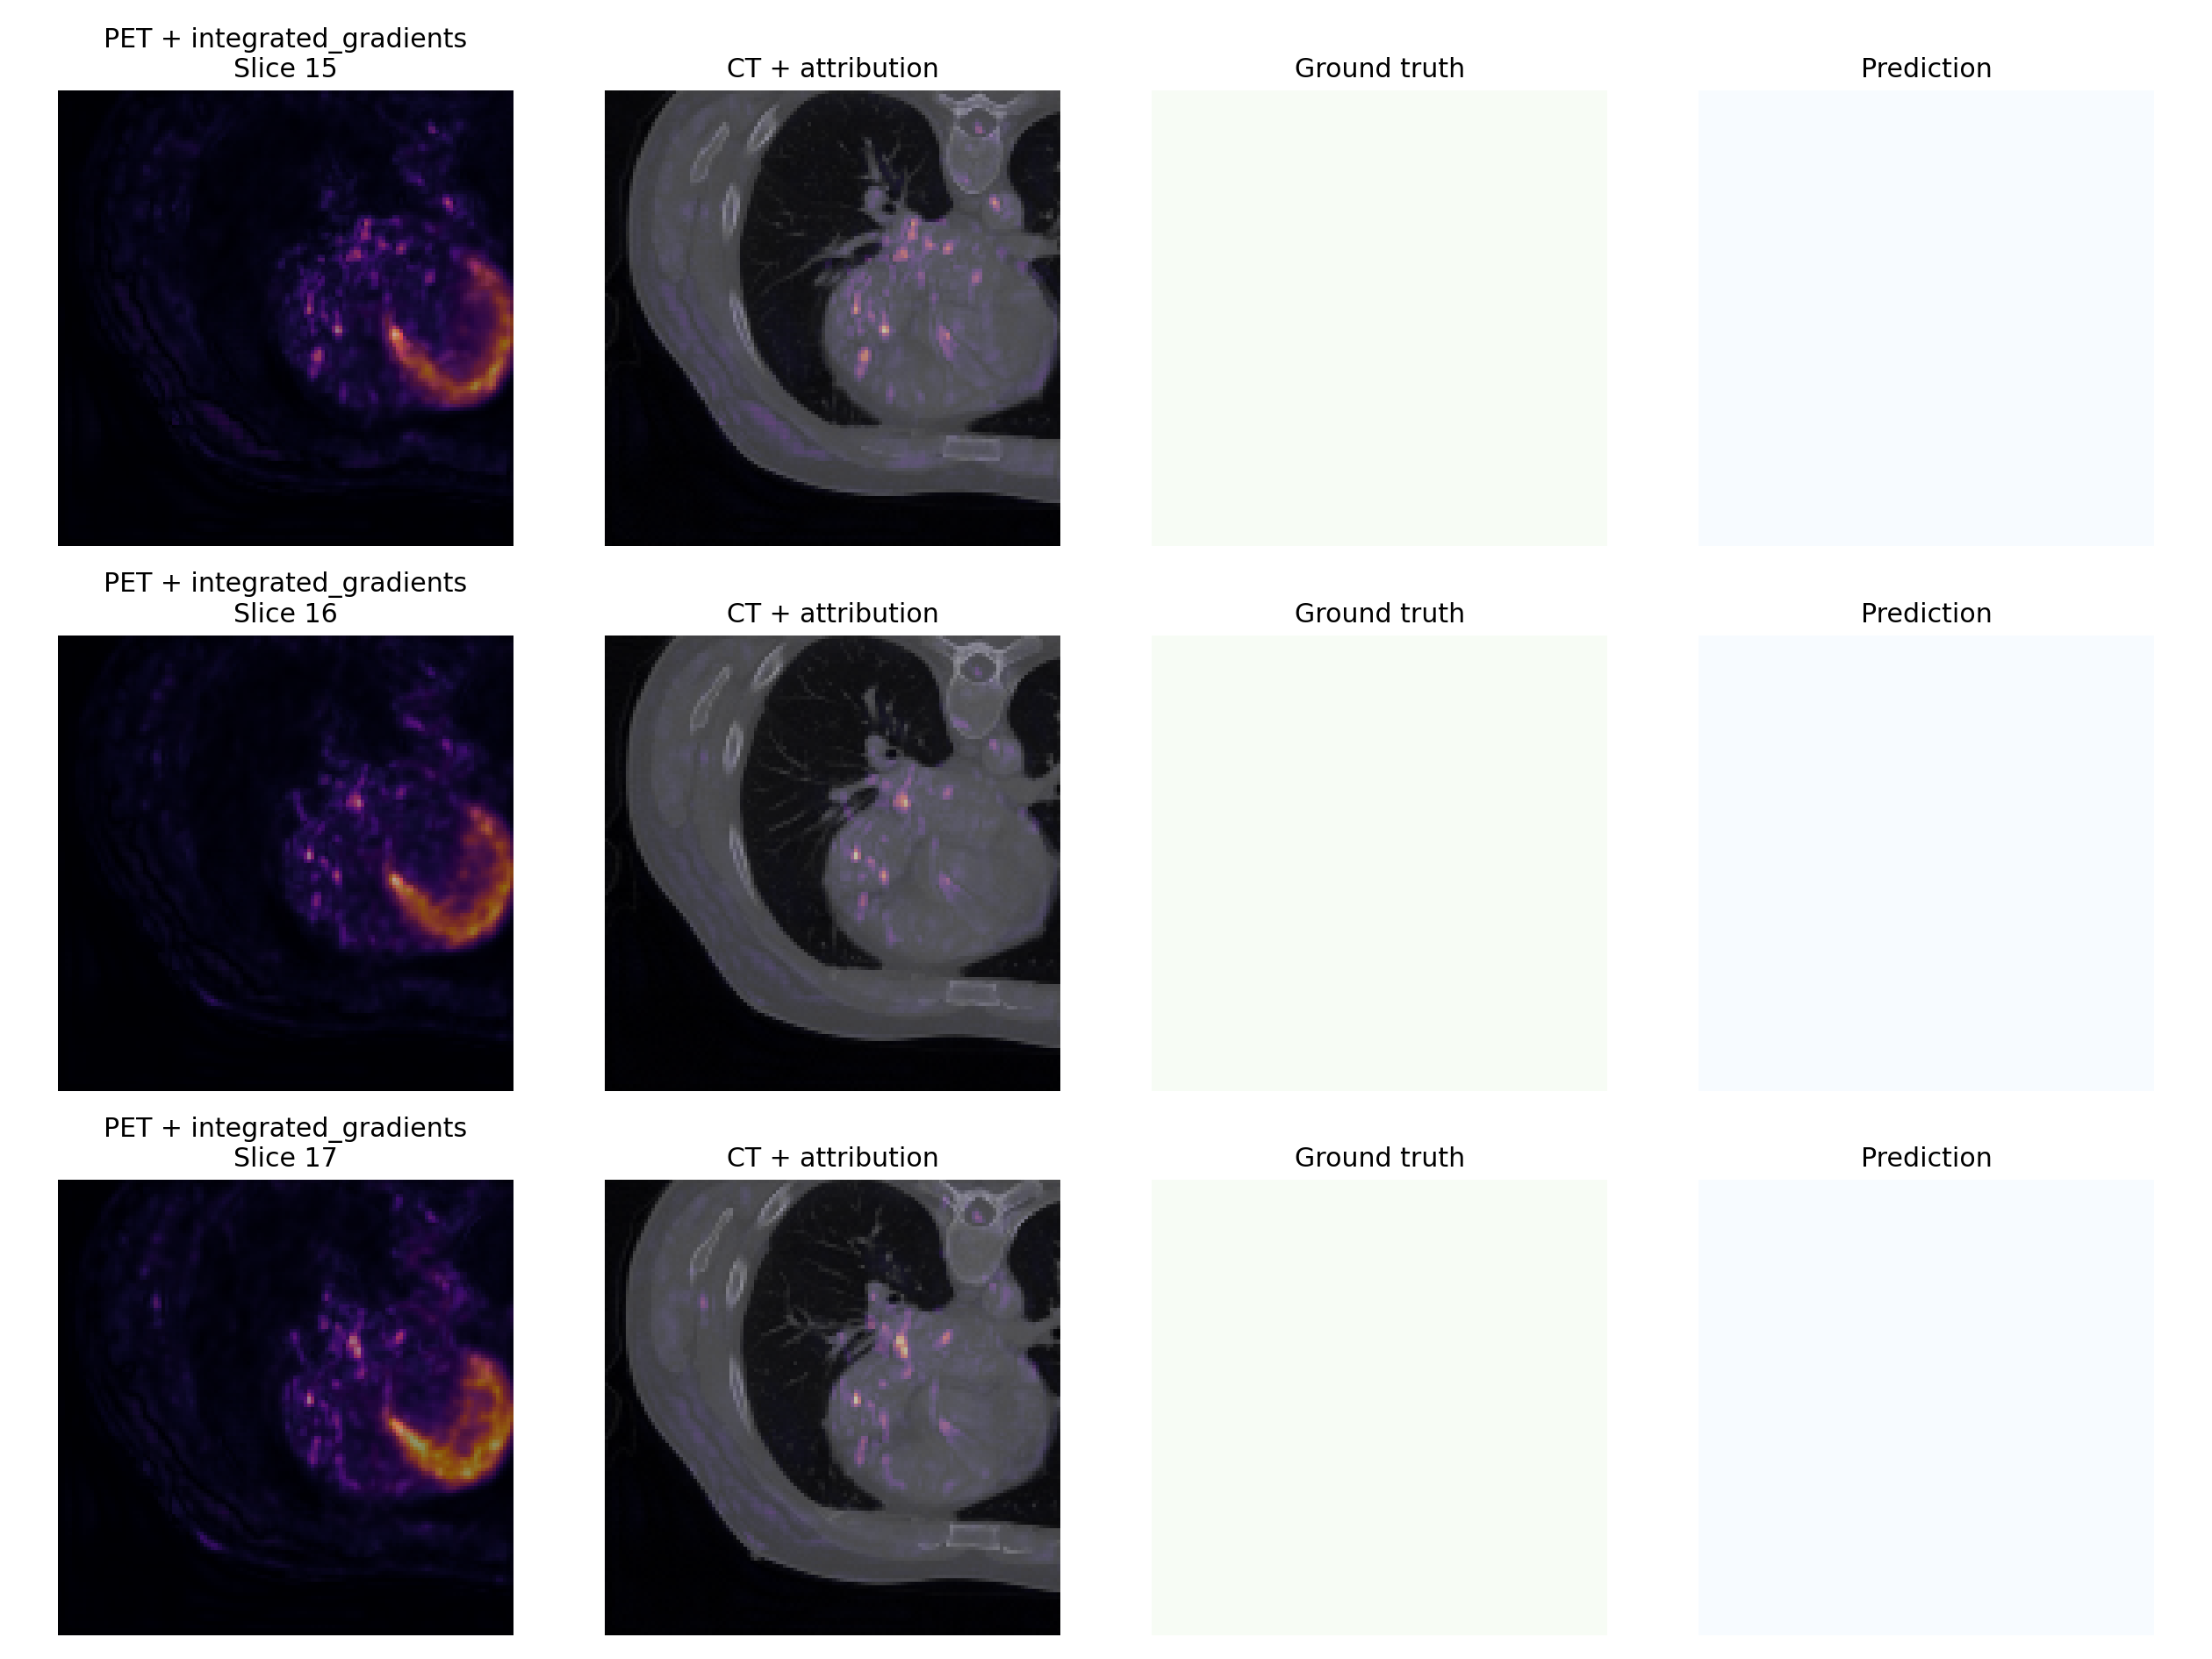
\includegraphics[width=0.86\linewidth]{../results/autopet_fdg_full_post_best_dice_50epochs_xai_allcases_20260327/figures/PETCT_a1db71e797/integrated_gradients.png}
\caption{Cas positif bien détecté avec Integrated Gradients. C'est l'exemple à garder pour montrer un cas où l'attribution suit la lésion.}
\end{figure}

\begin{figure}[htbp]
\centering
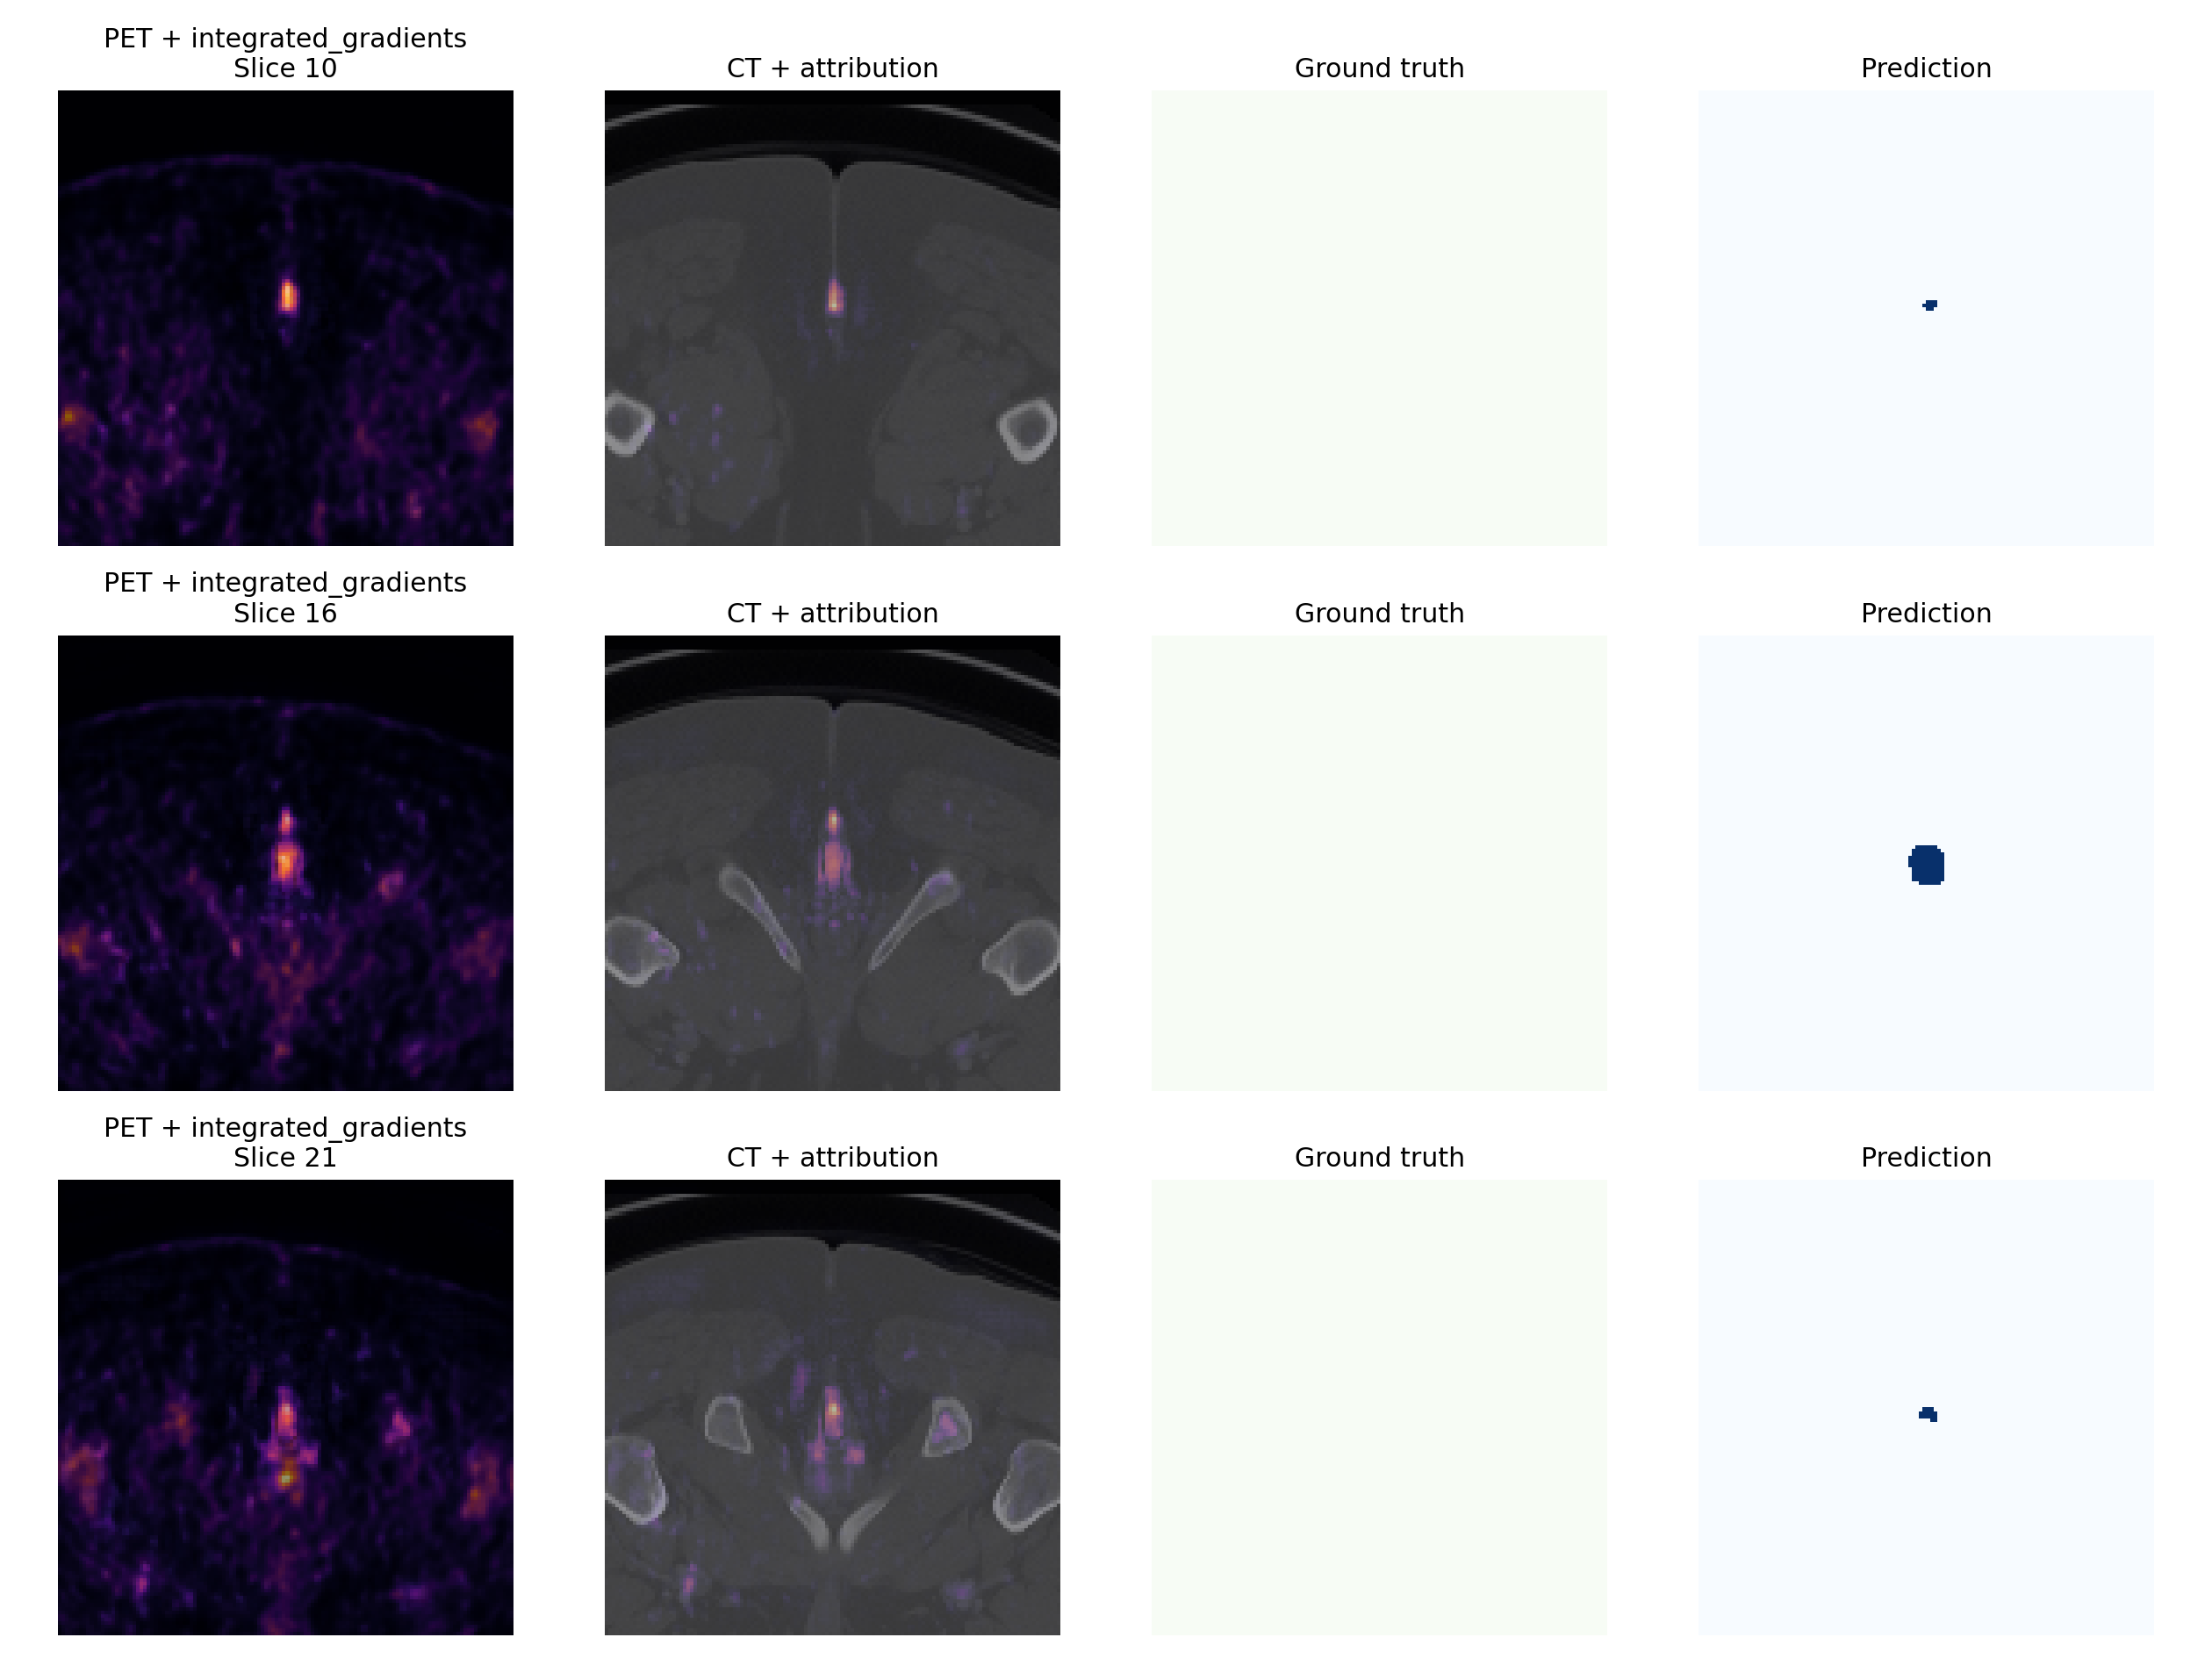
\includegraphics[width=0.86\linewidth]{../results/autopet_fdg_full_post_best_dice_50epochs_xai_allcases_20260327/figures/PETCT_05bed31780/integrated_gradients.png}
\caption{Cas faux positif avec Integrated Gradients. Cet exemple sert à expliquer pourquoi le modèle peut se tromper sur des structures non lésionnelles.}
\end{figure}

\begin{figure}[htbp]
\centering
\begin{tabular}{cc}
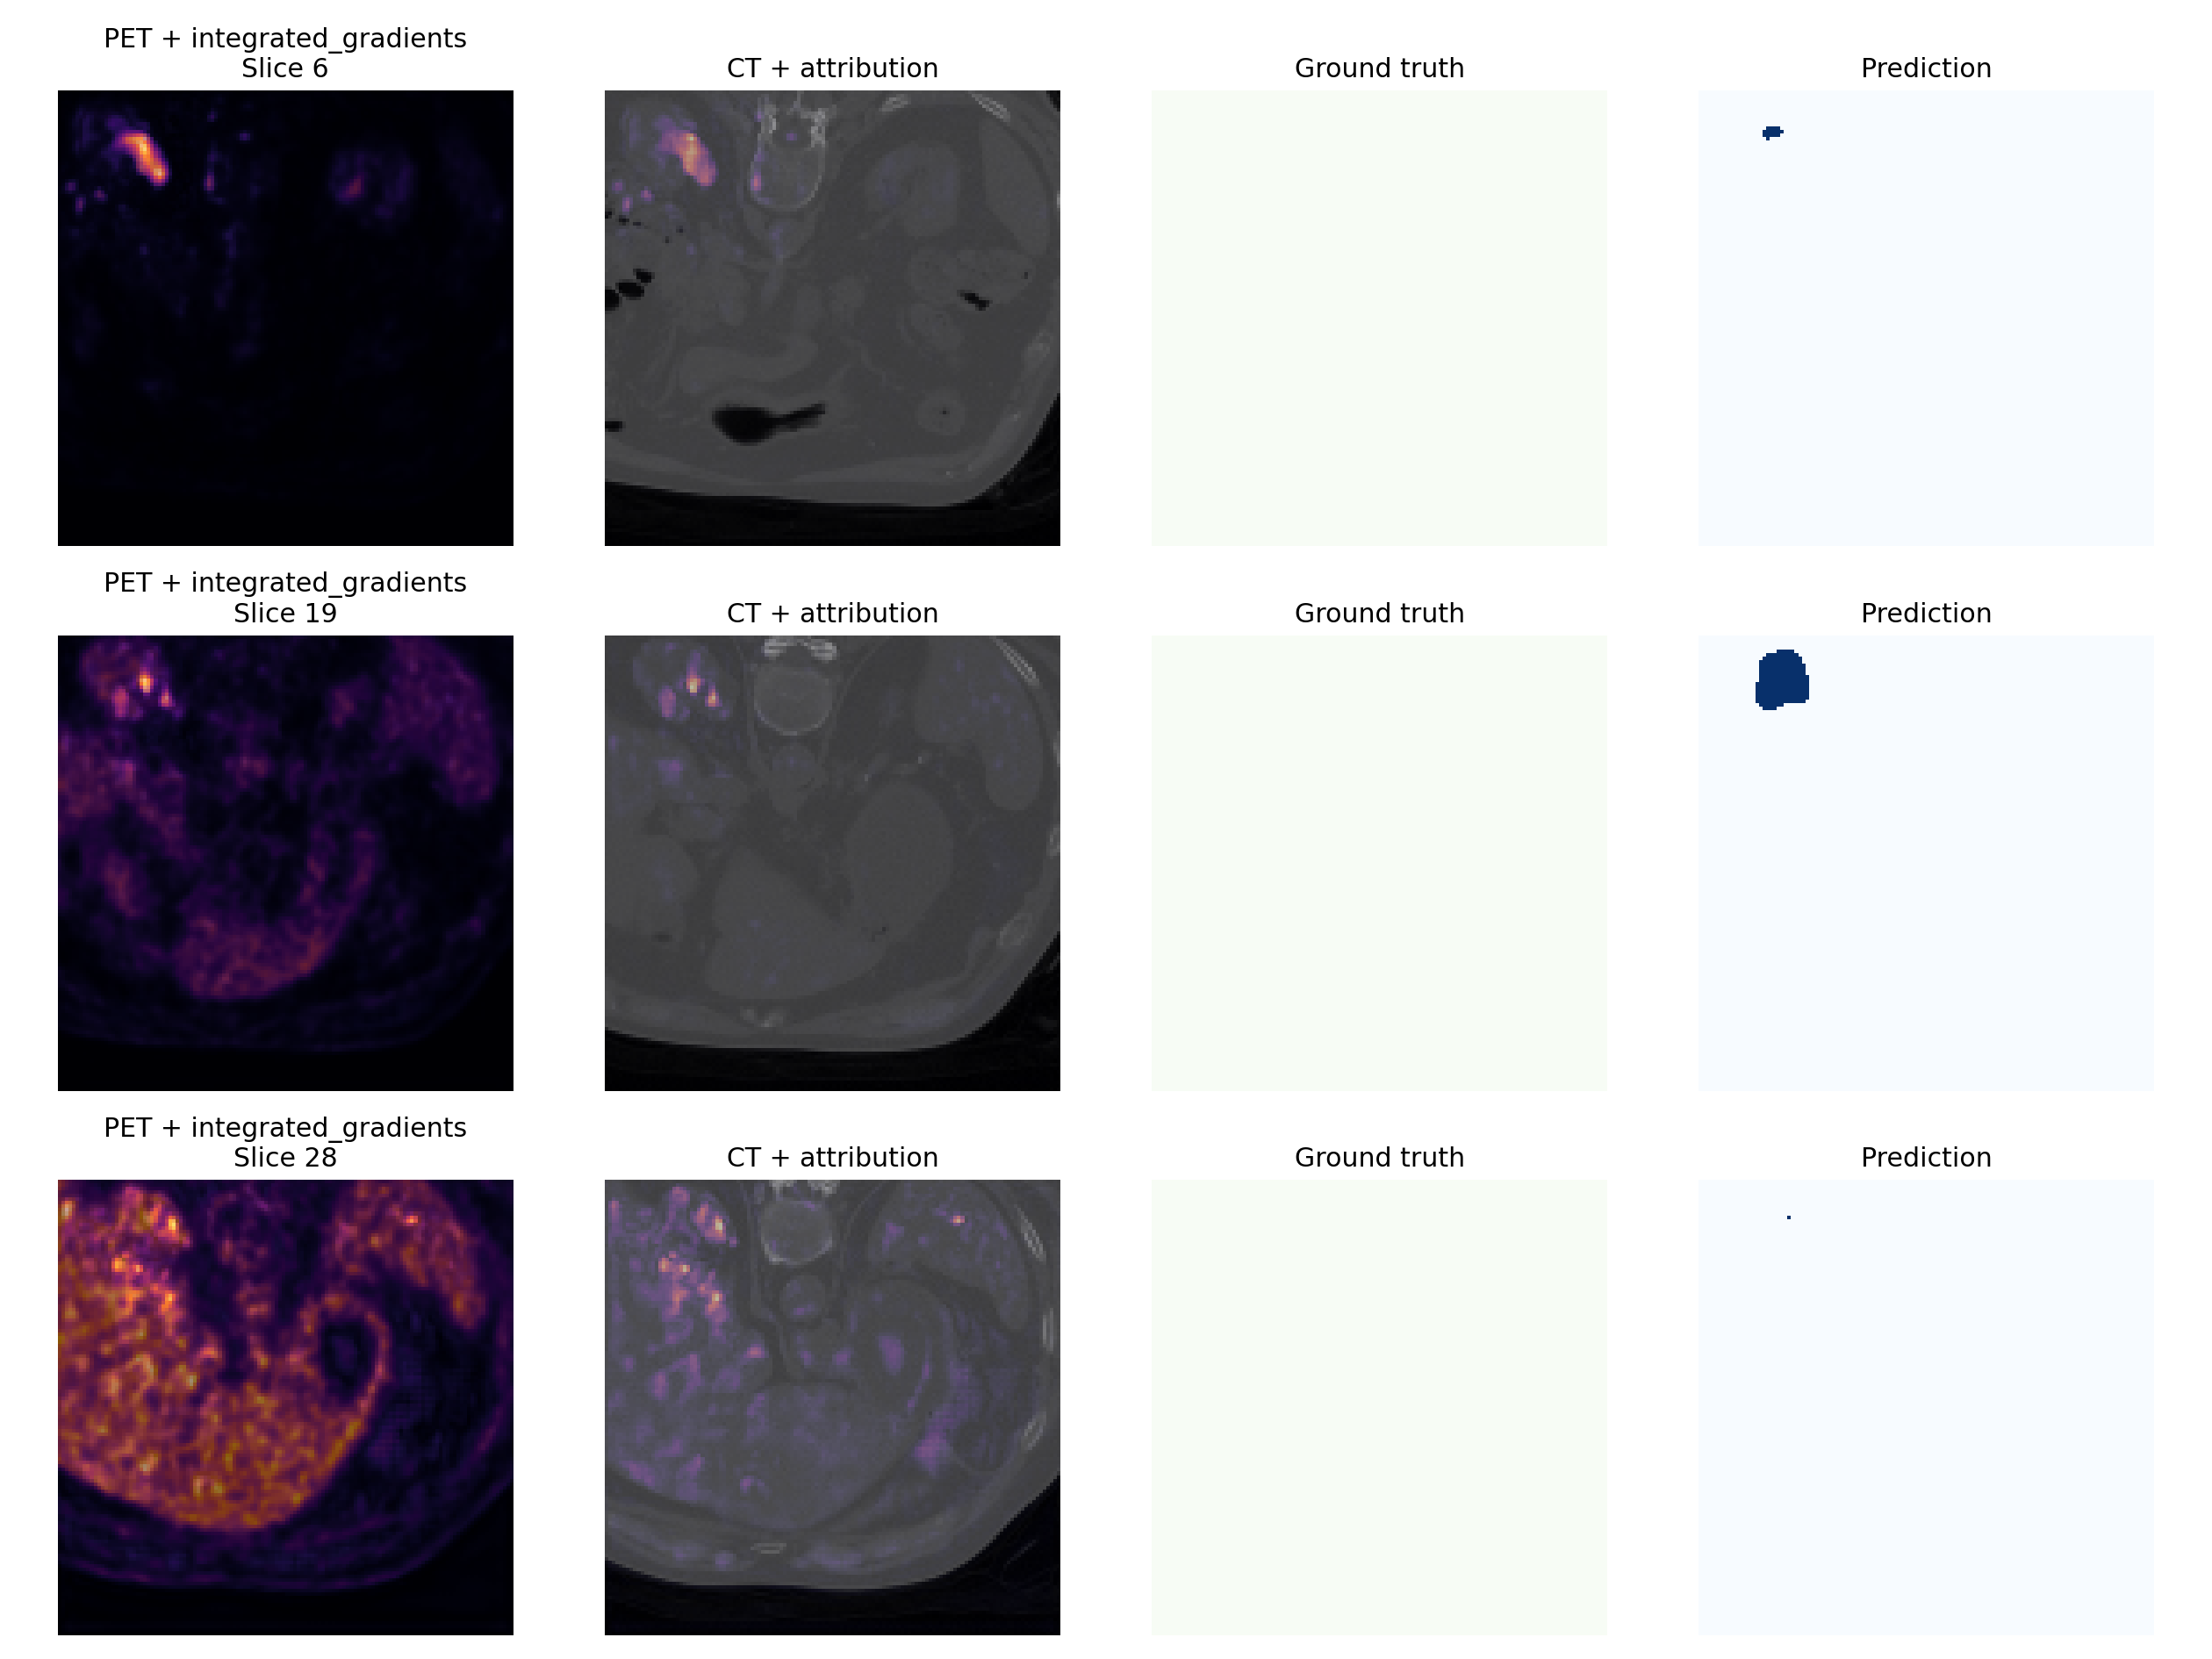
\includegraphics[width=0.46\linewidth]{../results/autopet_fdg_full_50epochs_variant_comparison_20260324/figures/raw_50epochs__PETCT_402c061122.png} &
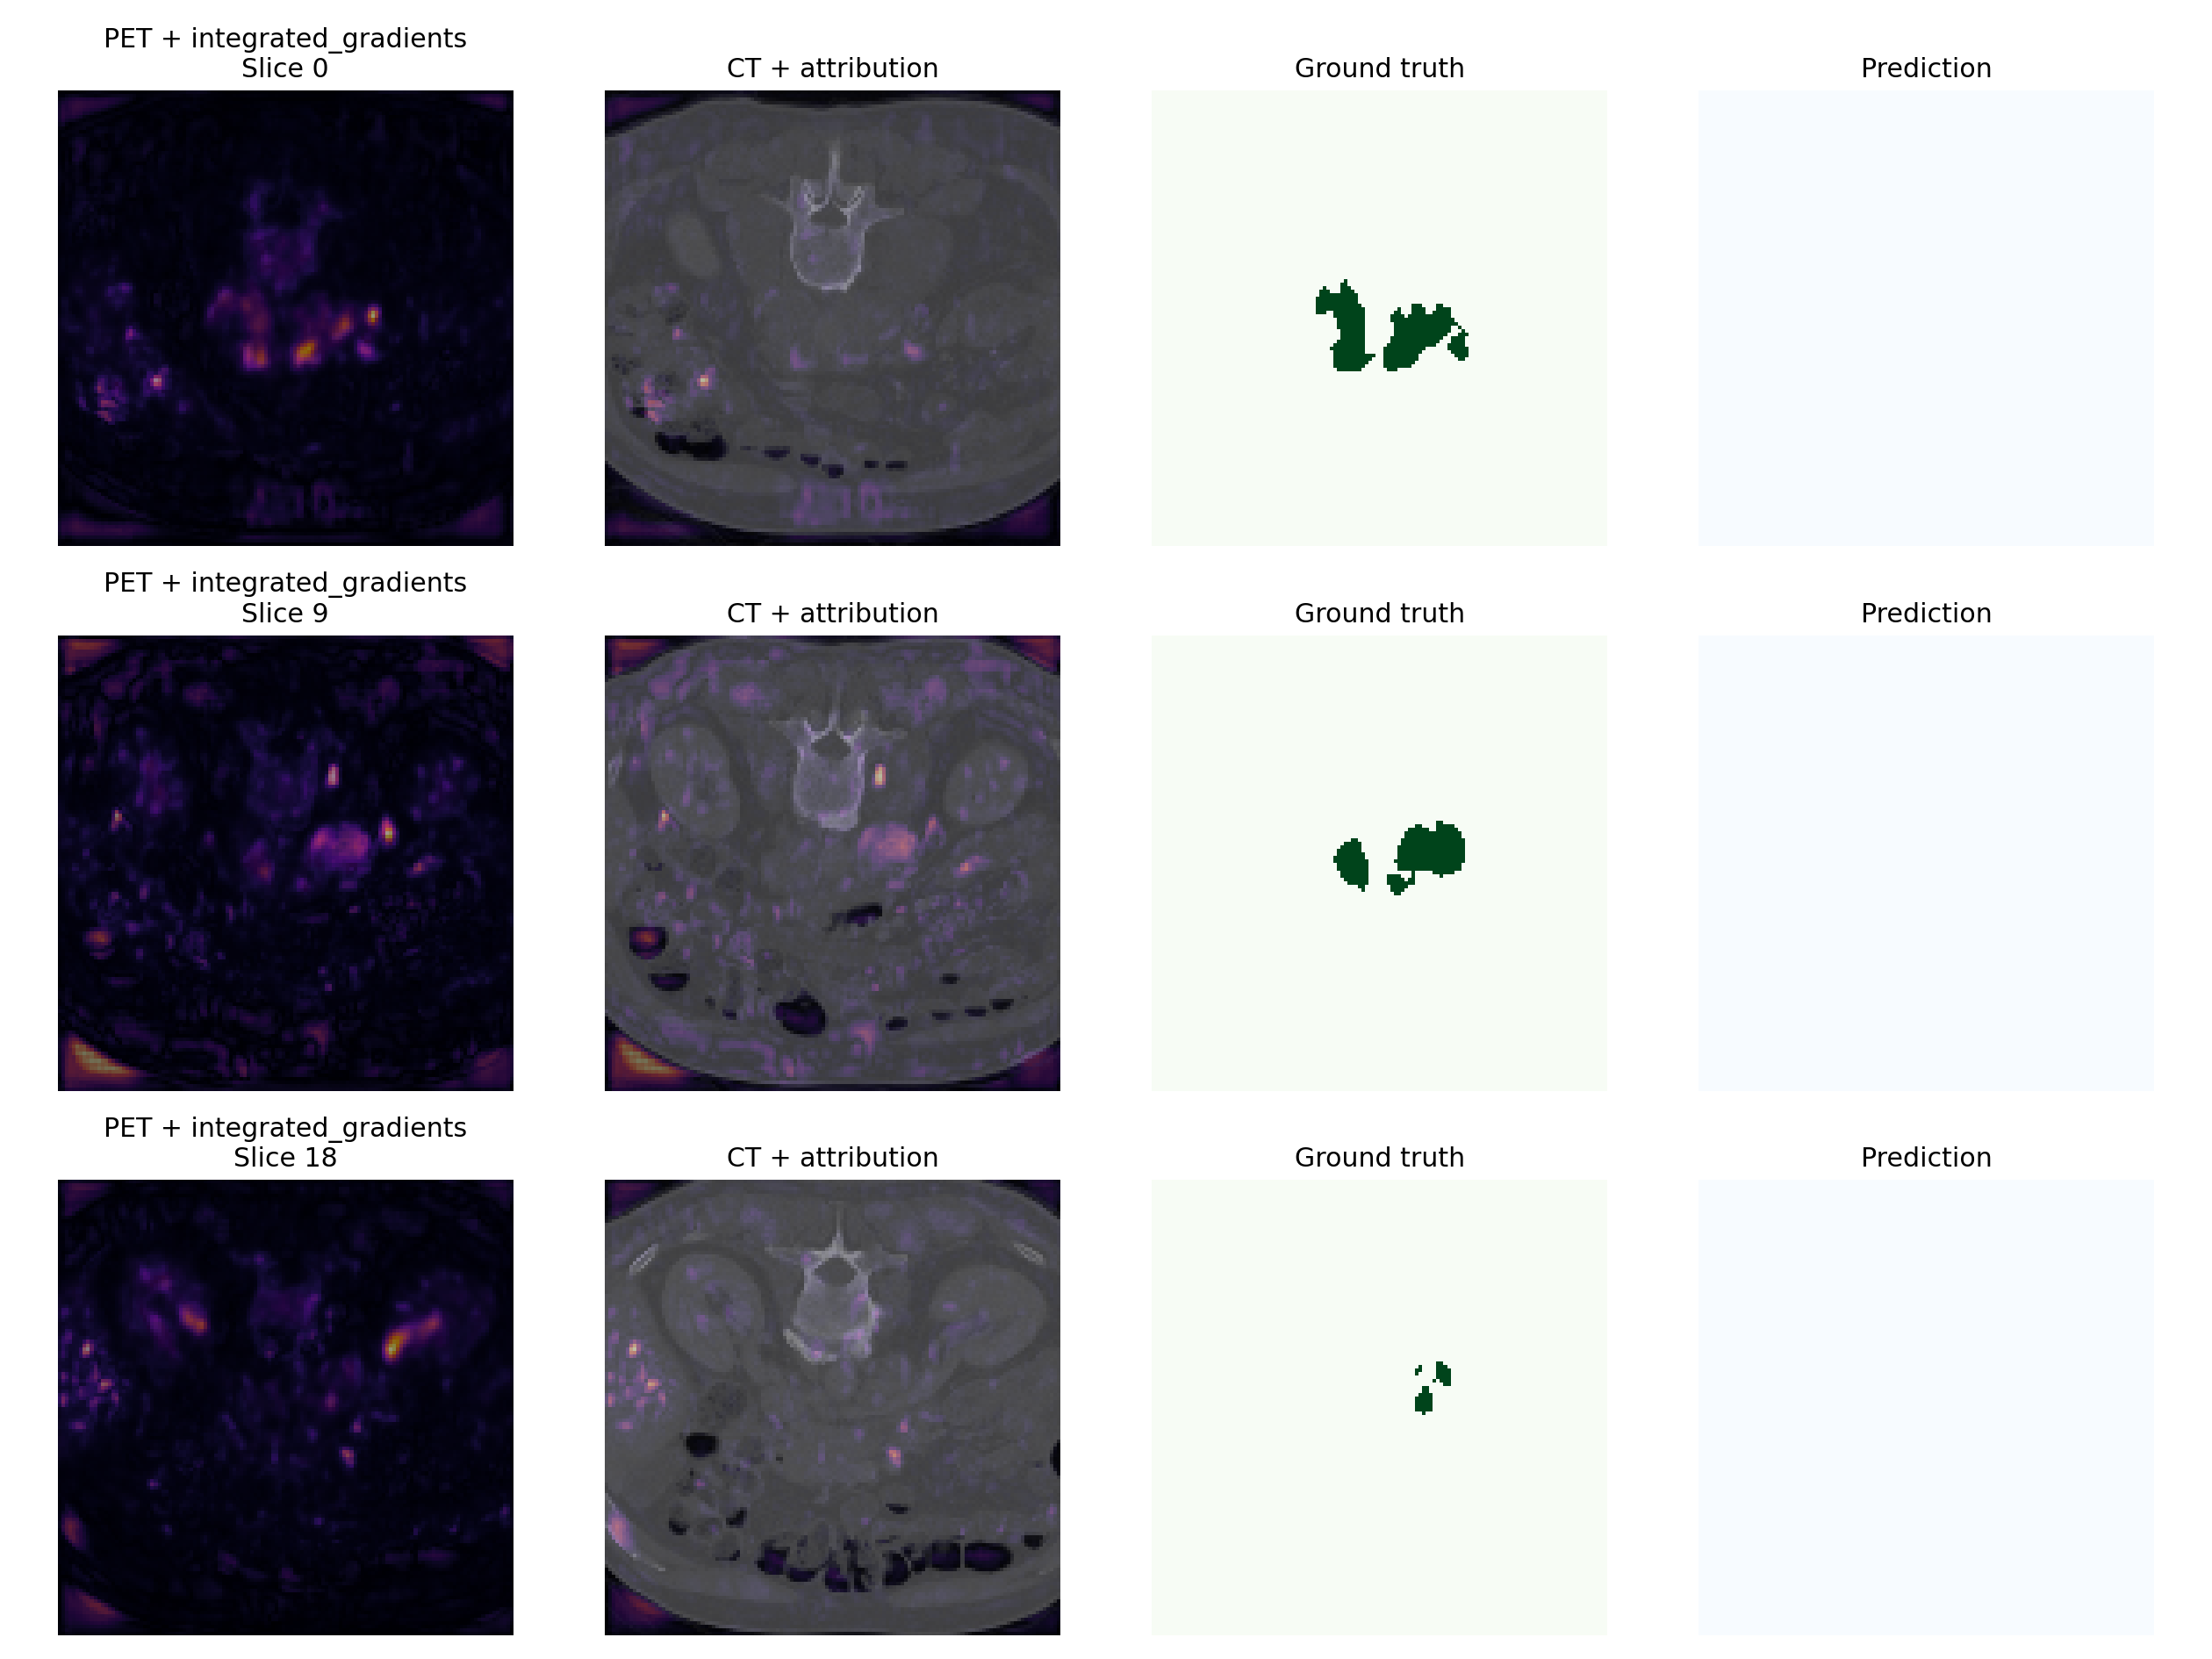
\includegraphics[width=0.46\linewidth]{../results/autopet_fdg_full_50epochs_variant_comparison_20260324/figures/raw_50epochs__PETCT_4848bebb10.png} \\
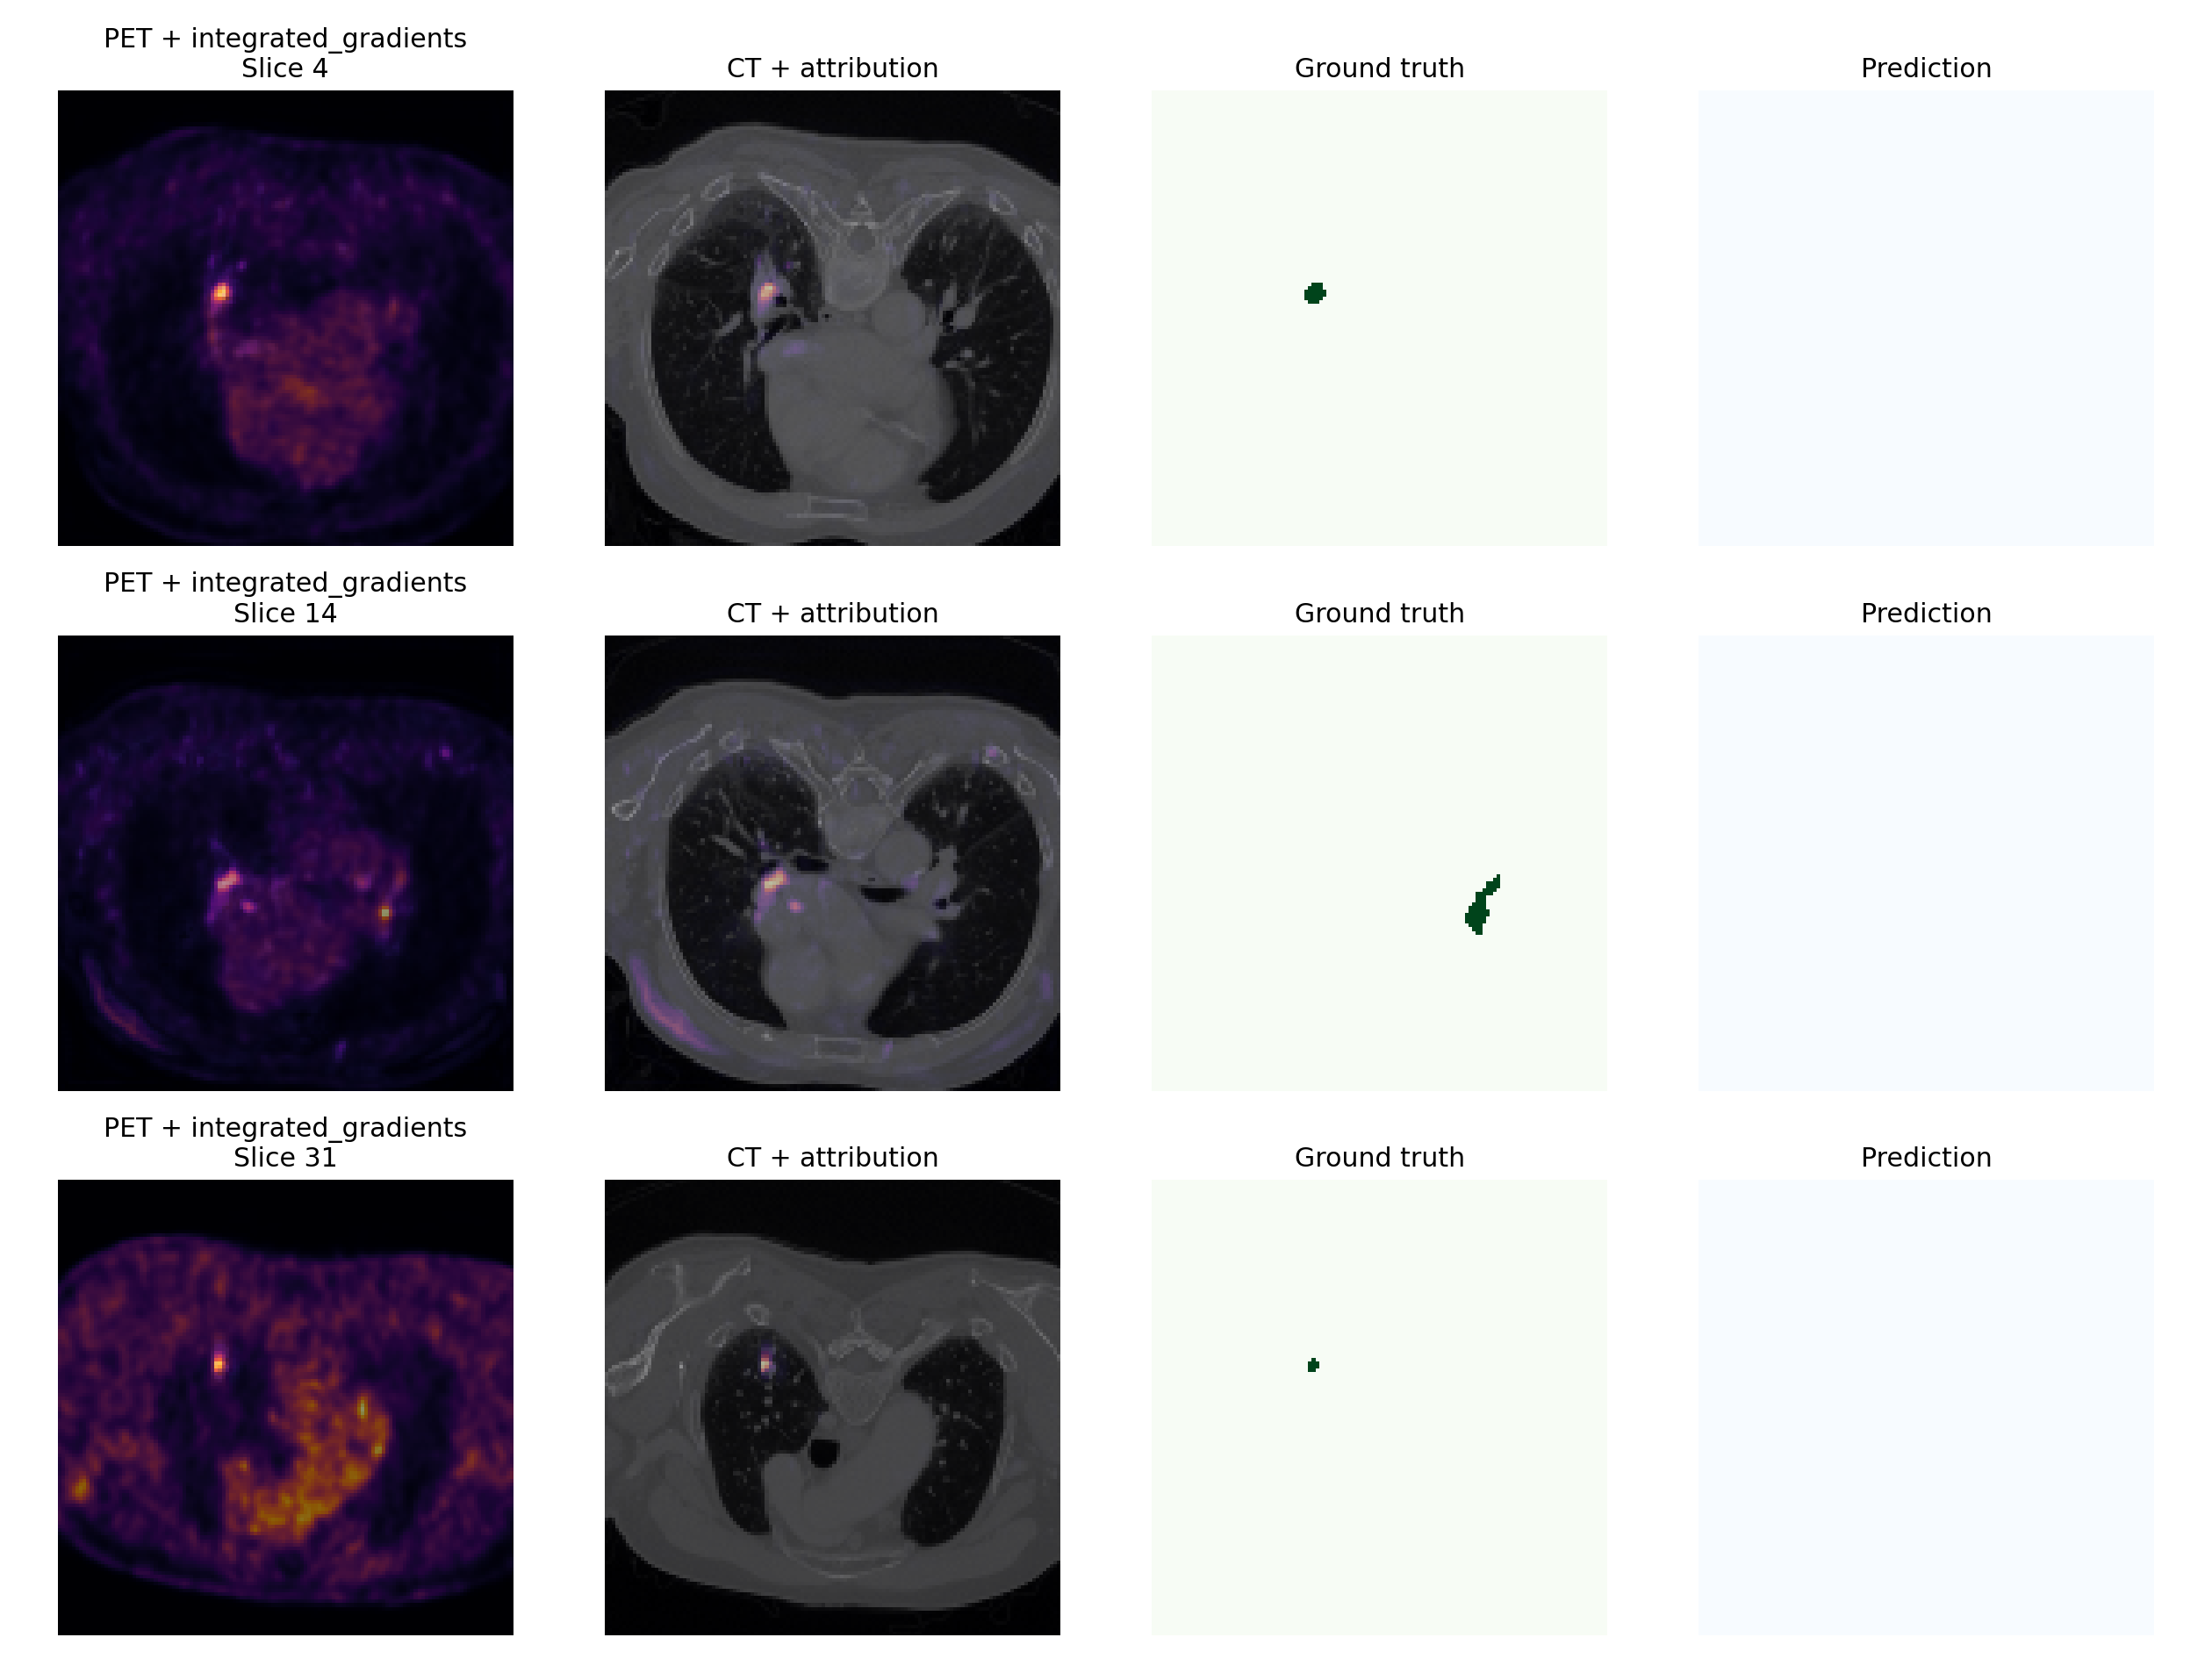
\includegraphics[width=0.46\linewidth]{../results/autopet_fdg_full_50epochs_variant_comparison_20260324/figures/post_best_dice_50epochs__PETCT_be3e55a32f.png} &
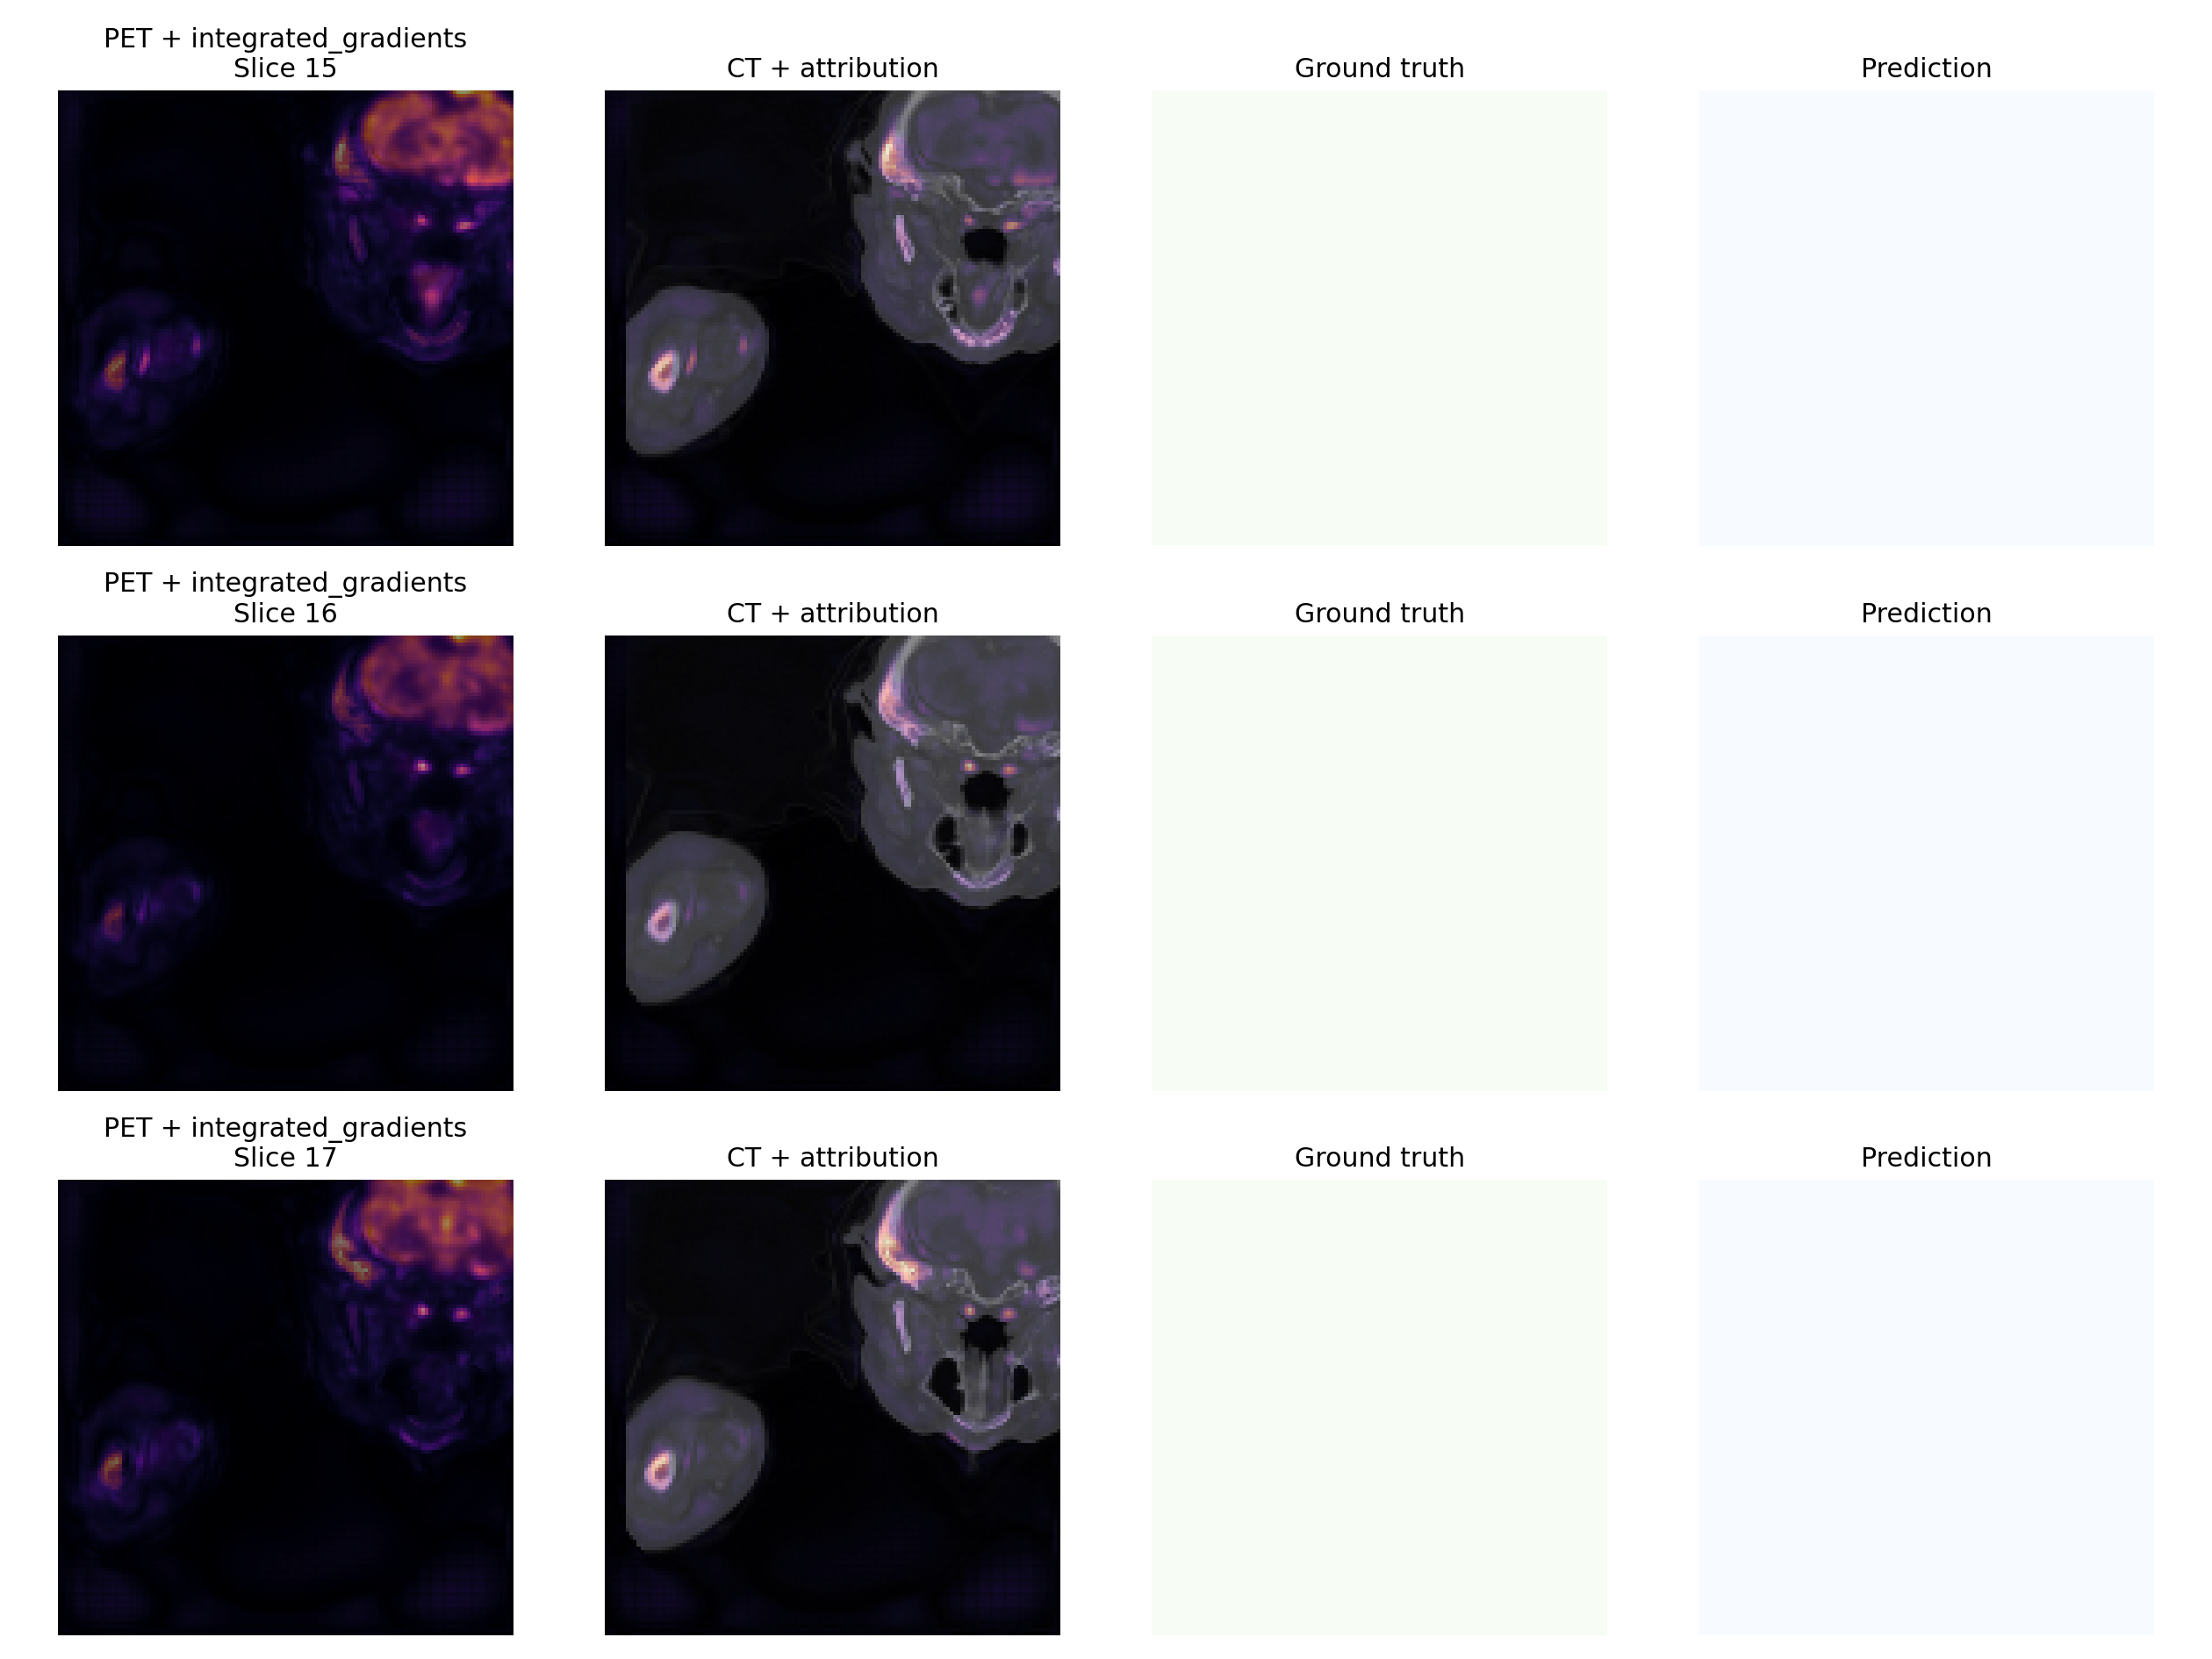
\includegraphics[width=0.46\linewidth]{../results/autopet_fdg_full_50epochs_variant_comparison_20260324/figures/post_low_fp_50epochs__PETCT_e2309b8f92.png}
\end{tabular}
\caption{Comparaison entre brut et post-traité sur quatre cas représentatifs. Le bloc du haut montre les cas bruts, le bloc du bas montre les variantes post-traitées.}
\end{figure}

\section{Partie de secours : Brain MRI}

Cette partie est la baseline de secours. Elle est plus simple que la piste
autoPET, mais elle reste utile pour garder un pipeline complet de classification
et pour disposer d'une seconde base de discussion plus rapide à relire.

\subsection{Ce qui a été gardé}

\begin{tabularx}{\linewidth}{L{5.1cm}Y}
\toprule
\textbf{Élément} & \textbf{Choix retenu} \\
\midrule
Donnée & Kaggle \texttt{Brain MRI tumor detection} \\
Tâche & Classification binaire \texttt{yes/no} \\
Modèle de base & \texttt{ResNet18} \\
Plateforme & Grid'5000 Grenoble \\
Résultat tracé & 5 à 6 époques selon les snapshots gardés \\
XAI & Grad-CAM, Integrated Gradients, Occlusion \\
\bottomrule
\end{tabularx}

\subsection{Résultats à citer}

\begin{tabularx}{\linewidth}{L{5.0cm}L{4.8cm}}
\toprule
\textbf{Métrique} & \textbf{Valeur} \\
\midrule
Accuracy & 0.8684 \\
Precision & 0.9091 \\
Recall & 0.8696 \\
F1 & 0.8889 \\
ROC-AUC & 0.9391 \\
\bottomrule
\end{tabularx}

La matrice de confusion associée est \texttt{[[13, 2], [3, 20]]}. En pratique,
cela veut dire que le modèle se trompe encore un peu sur les images négatives,
mais qu'il reste globalement solide pour cette baseline de secours.

\subsection{Figures utiles}

\begin{figure}[htbp]
\centering
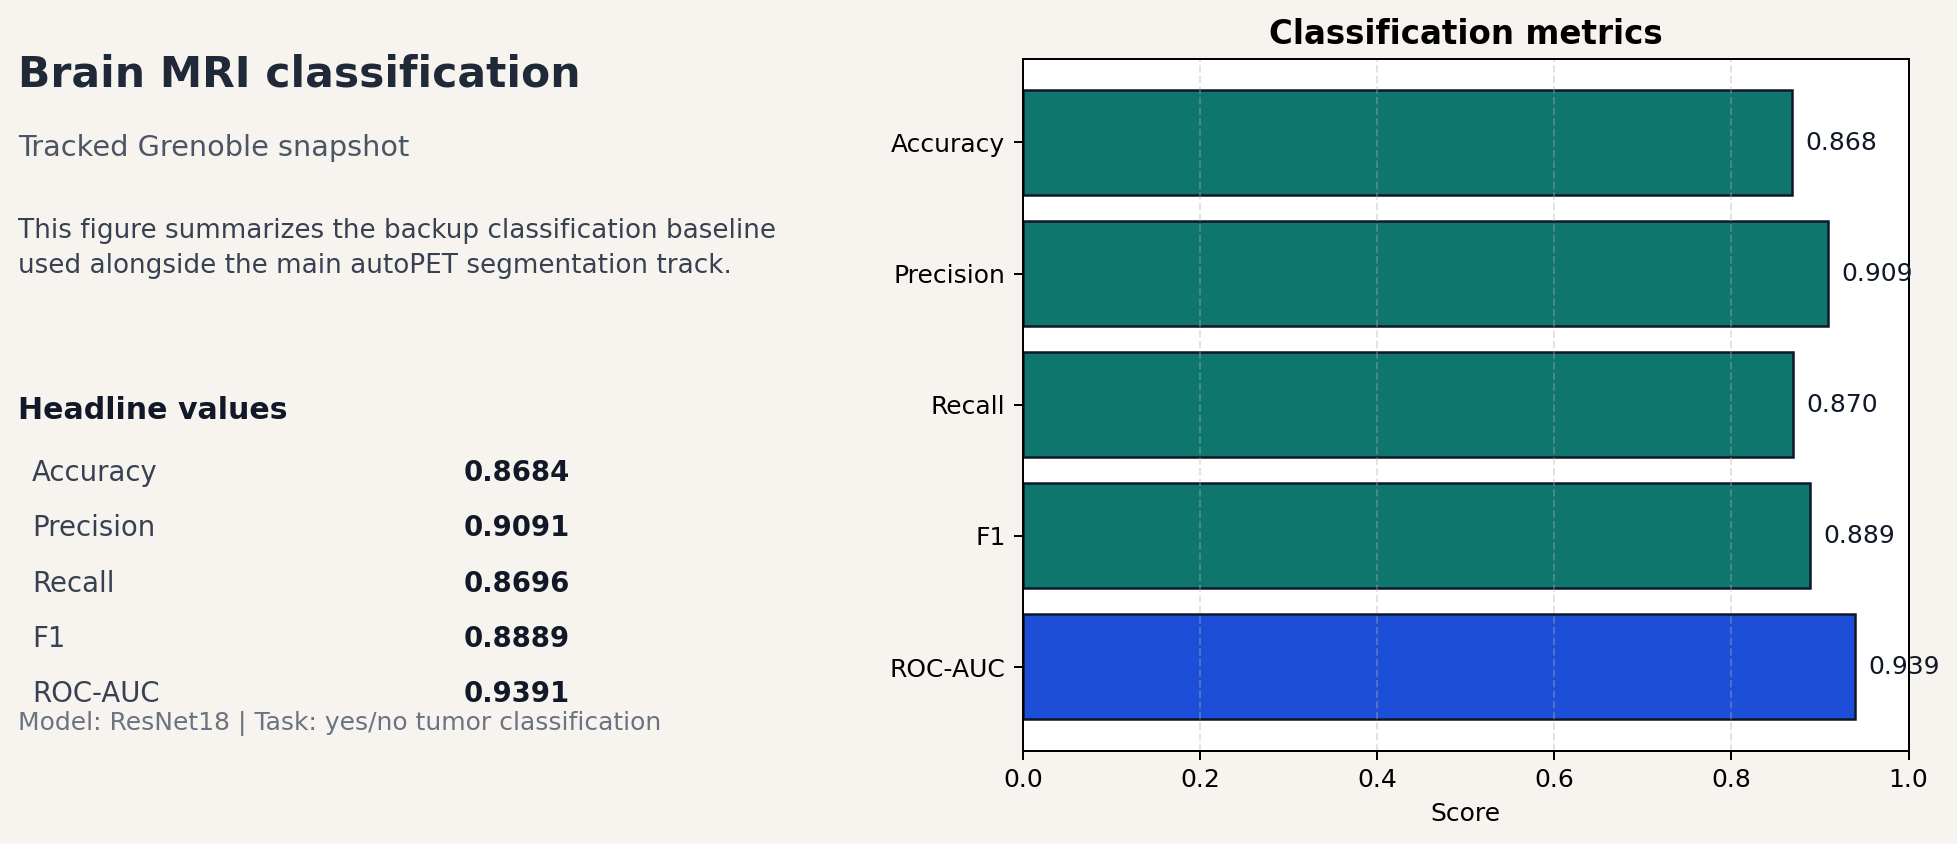
\includegraphics[width=0.92\linewidth]{../results/grenoble_gpu_20260324/figures/metrics_overview.png}
\caption{Vue d'ensemble du run Brain MRI. Cette figure suffit pour présenter les métriques principales sans entrer dans les détails du training.}
\end{figure}

\begin{figure}[htbp]
\centering
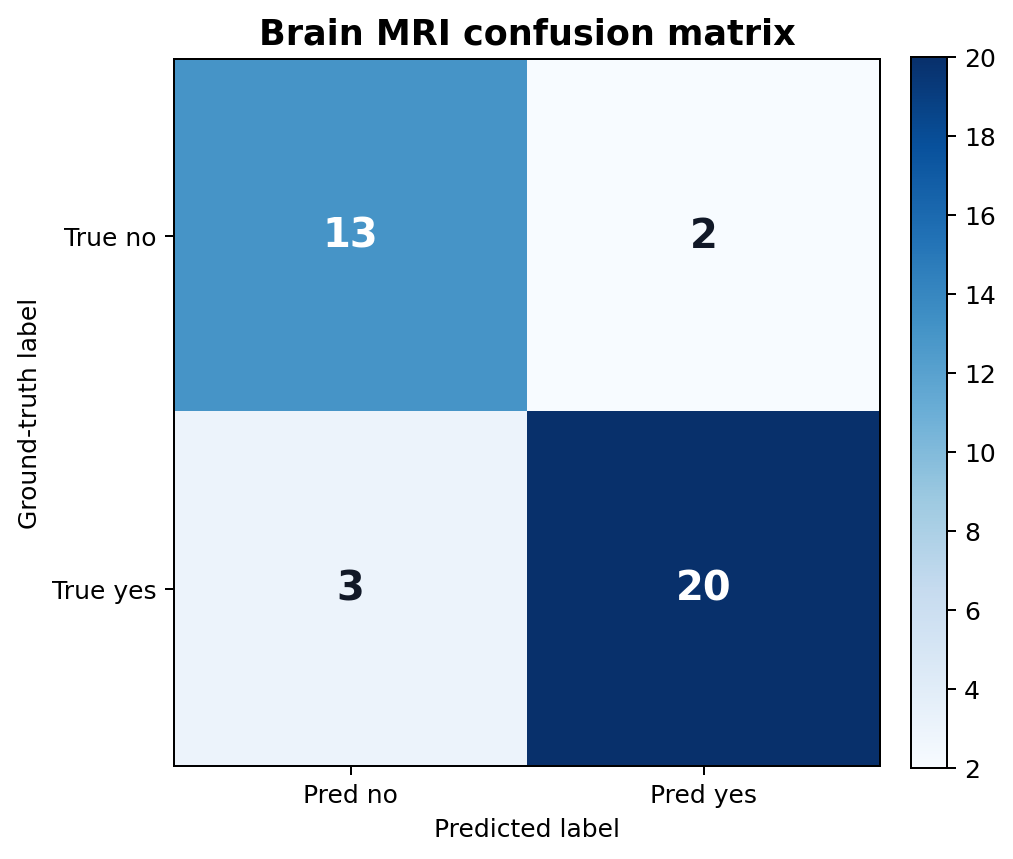
\includegraphics[width=0.58\linewidth]{../results/grenoble_gpu_20260324/figures/confusion_matrix.png}
\caption{Matrice de confusion Brain MRI. Elle sert de repère rapide pour voir le niveau d'erreur du modèle.}
\end{figure}

\begin{figure}[htbp]
\centering
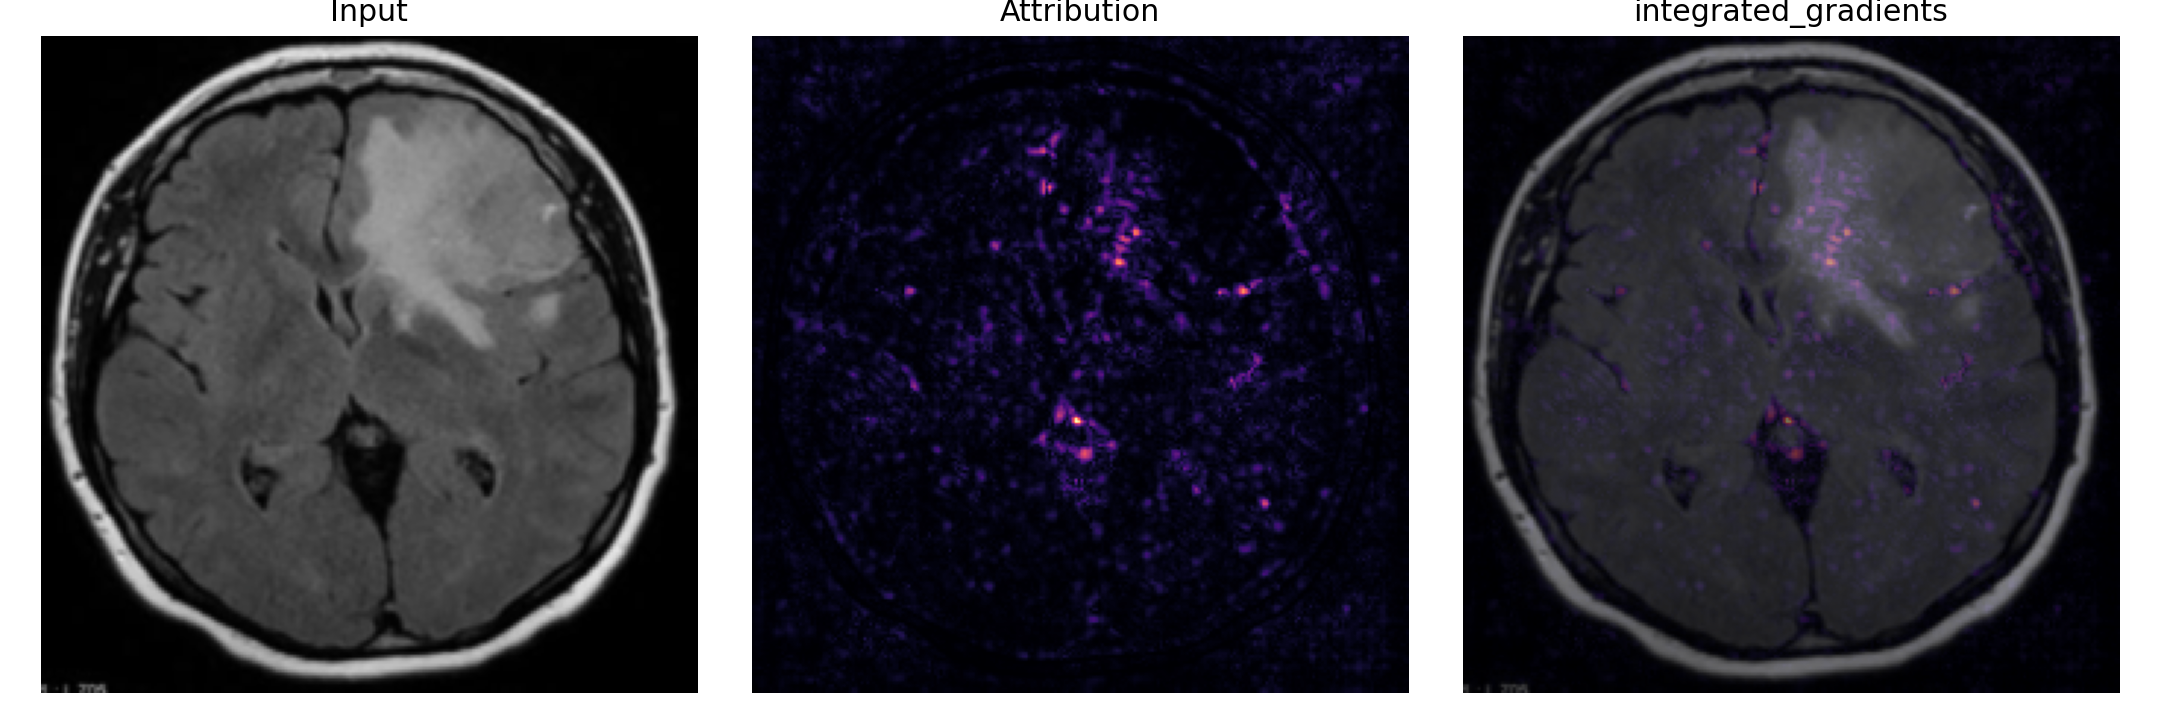
\includegraphics[width=0.46\linewidth]{../results/grenoble_gpu_20260324/xai/yes/Y195/integrated_gradients.png}\hfill
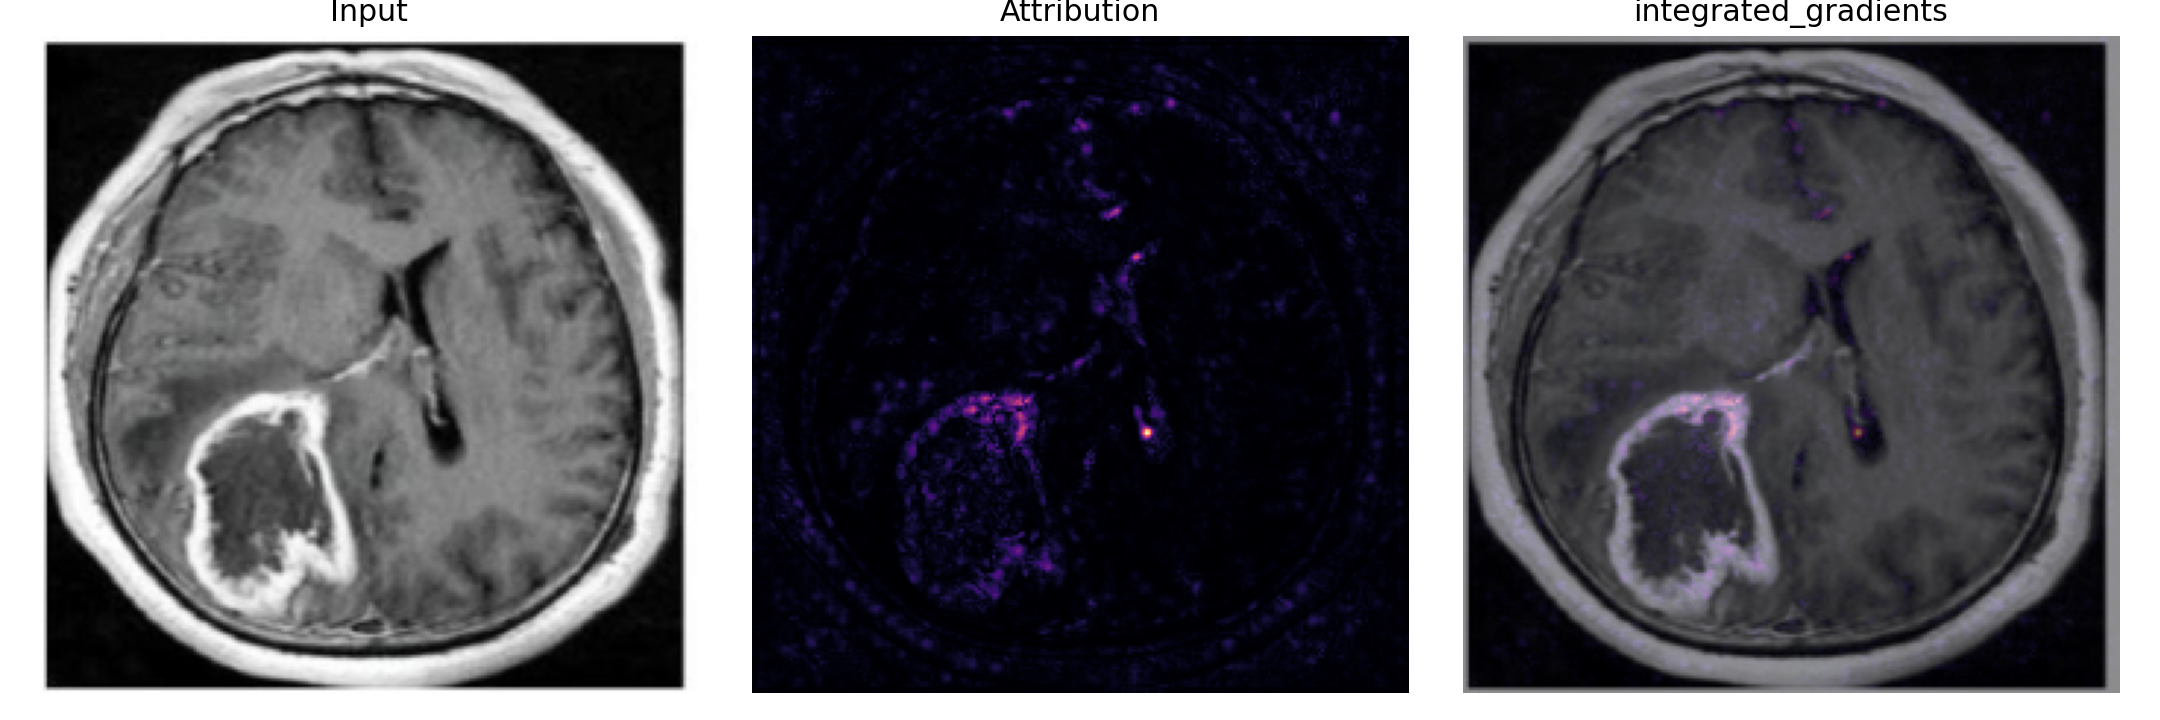
\includegraphics[width=0.46\linewidth]{../results/grenoble_gpu_20260324/xai/yes/Y109/integrated_gradients.png}
\vspace{0.4em}
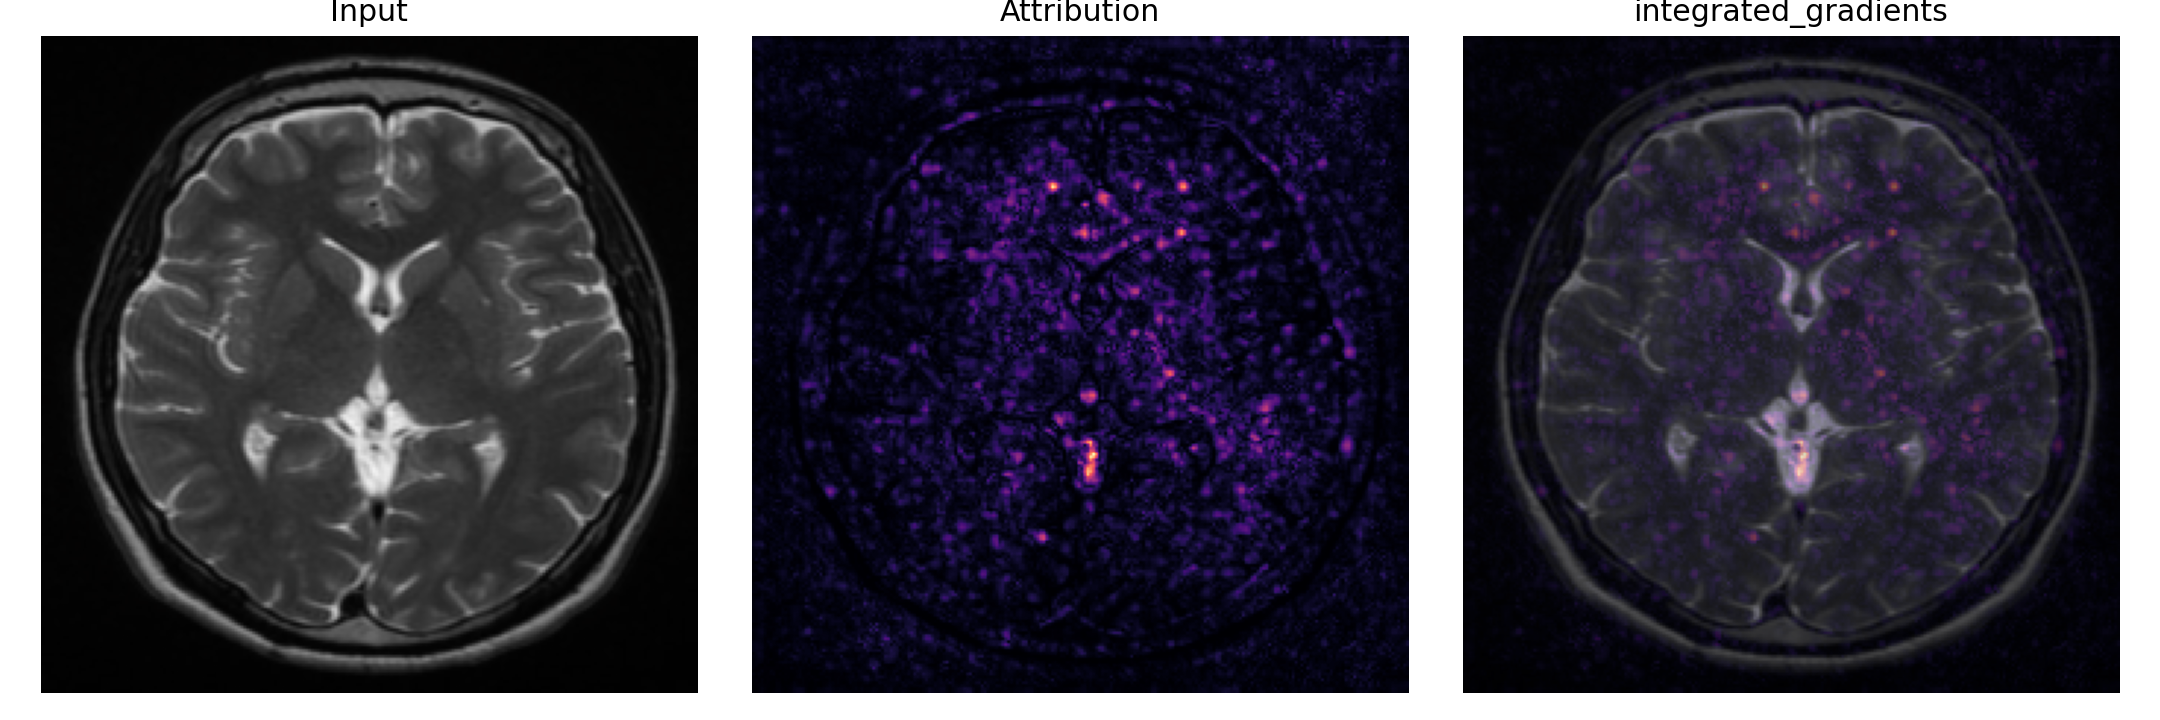
\includegraphics[width=0.46\linewidth]{../results/grenoble_gpu_20260324/xai/no/No22/integrated_gradients.png}\hfill

\includegraphics[width=0.46\linewidth]{\detokenize{../results/grenoble_gpu_20260324/xai/no/4 no/integrated_gradients.png}}
\caption{Exemples Brain MRI avec Integrated Gradients. Les cas positifs montrent où le modèle s'appuie pour prédire une tumeur, et les cas négatifs servent de contraste.}
\end{figure}

\begin{figure}[htbp]
\centering
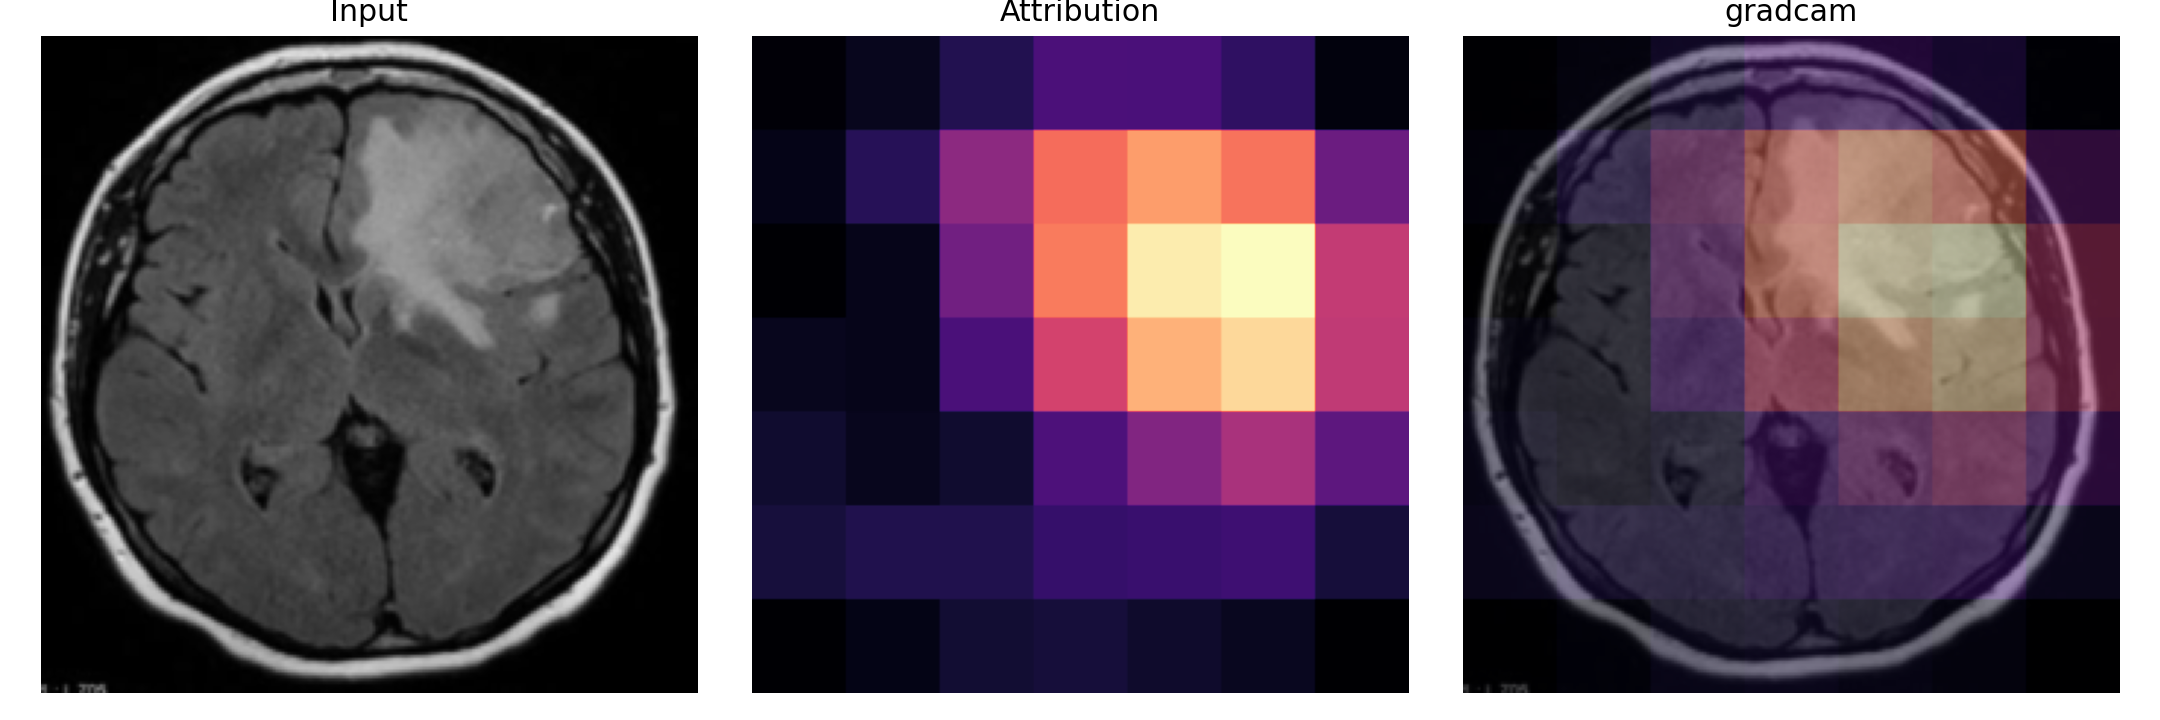
\includegraphics[width=0.46\linewidth]{../results/grenoble_gpu_20260324/xai/yes/Y195/gradcam.png}\hfill
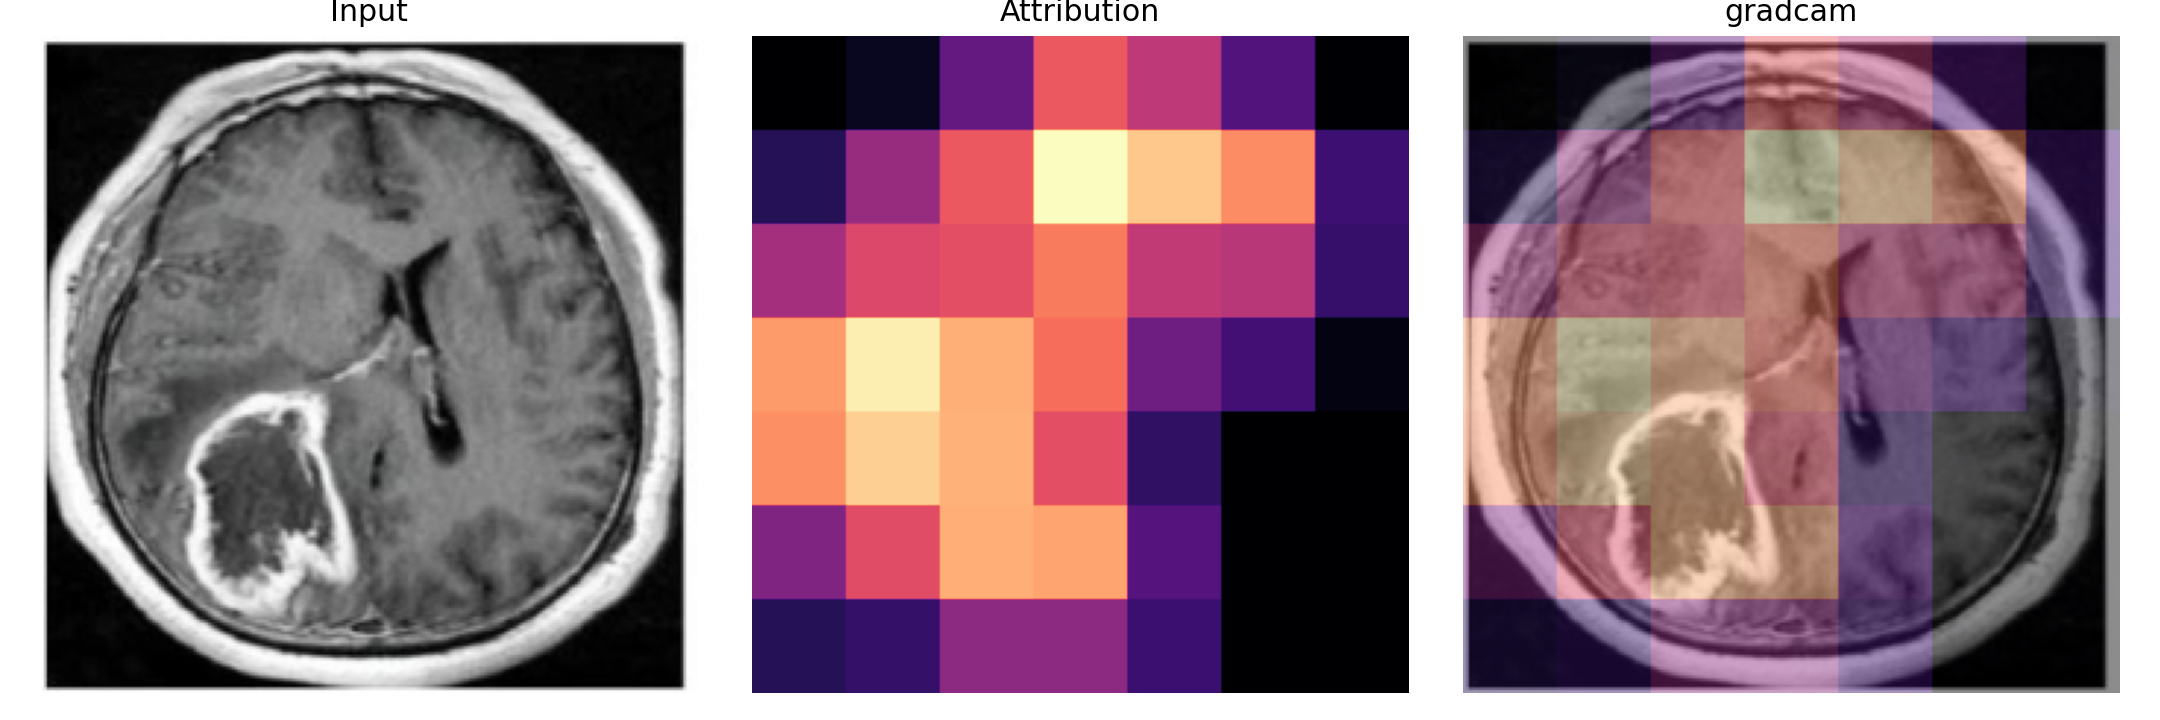
\includegraphics[width=0.46\linewidth]{../results/grenoble_gpu_20260324/xai/yes/Y109/gradcam.png}
\vspace{0.4em}
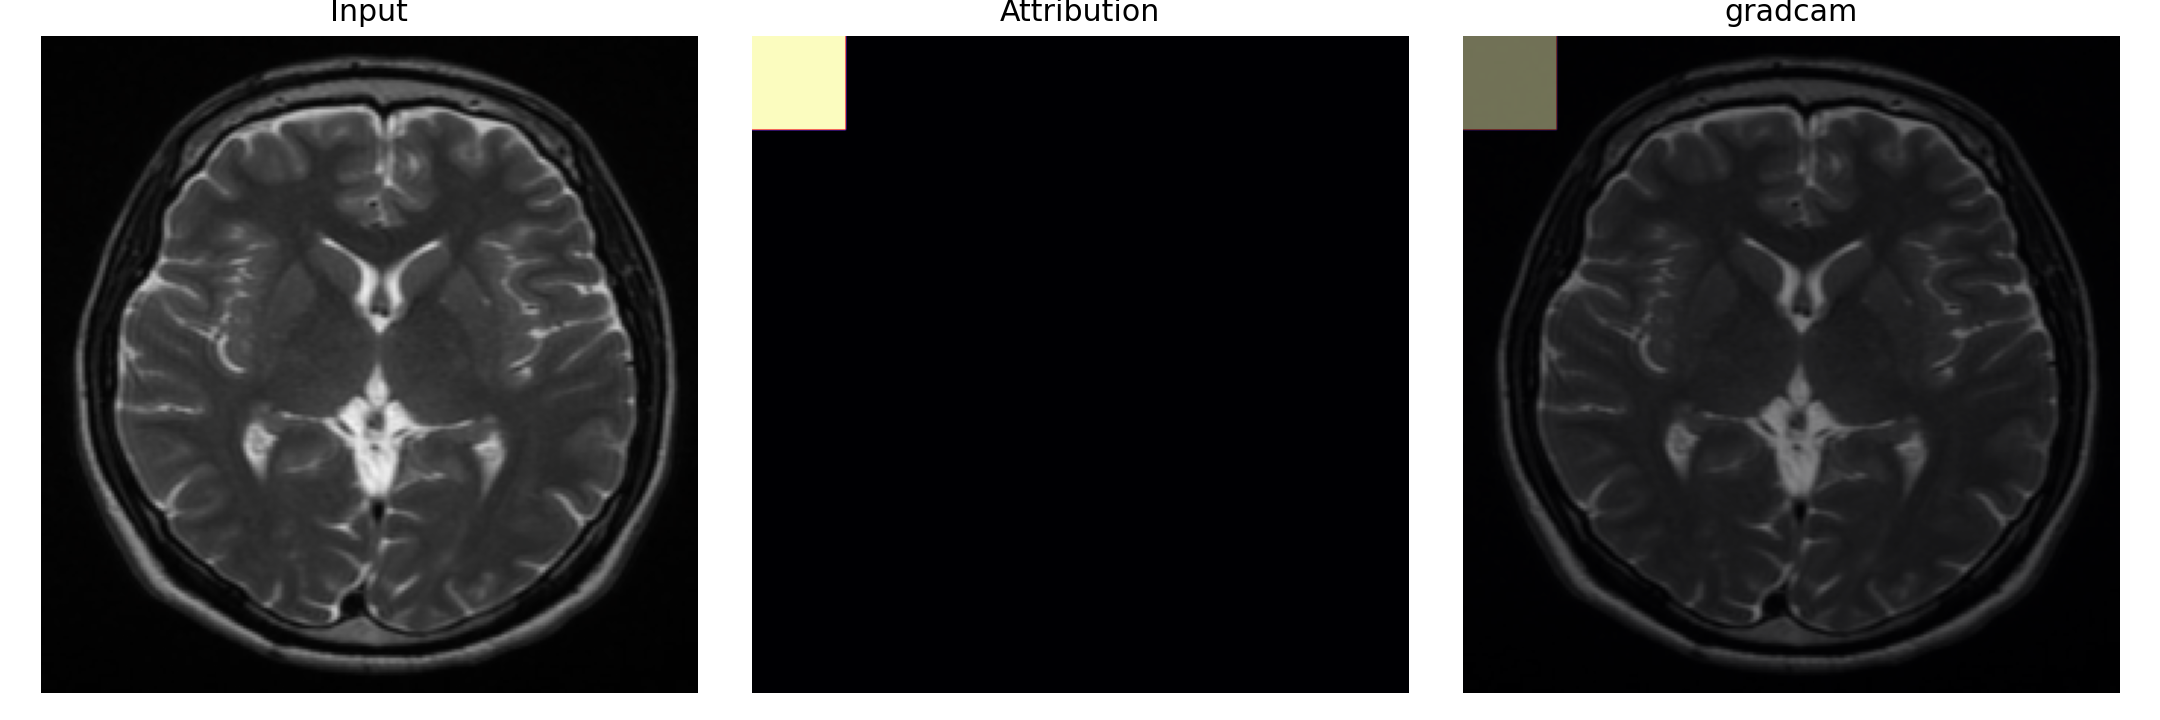
\includegraphics[width=0.46\linewidth]{../results/grenoble_gpu_20260324/xai/no/No22/gradcam.png}\hfill

\includegraphics[width=0.46\linewidth]{\detokenize{../results/grenoble_gpu_20260324/xai/no/4 no/gradcam.png}}
\caption{Même série Brain MRI avec Grad-CAM. C'est utile si l'équipe veut une méthode visuelle plus classique à commenter.}
\end{figure}

\begin{figure}[htbp]
\centering
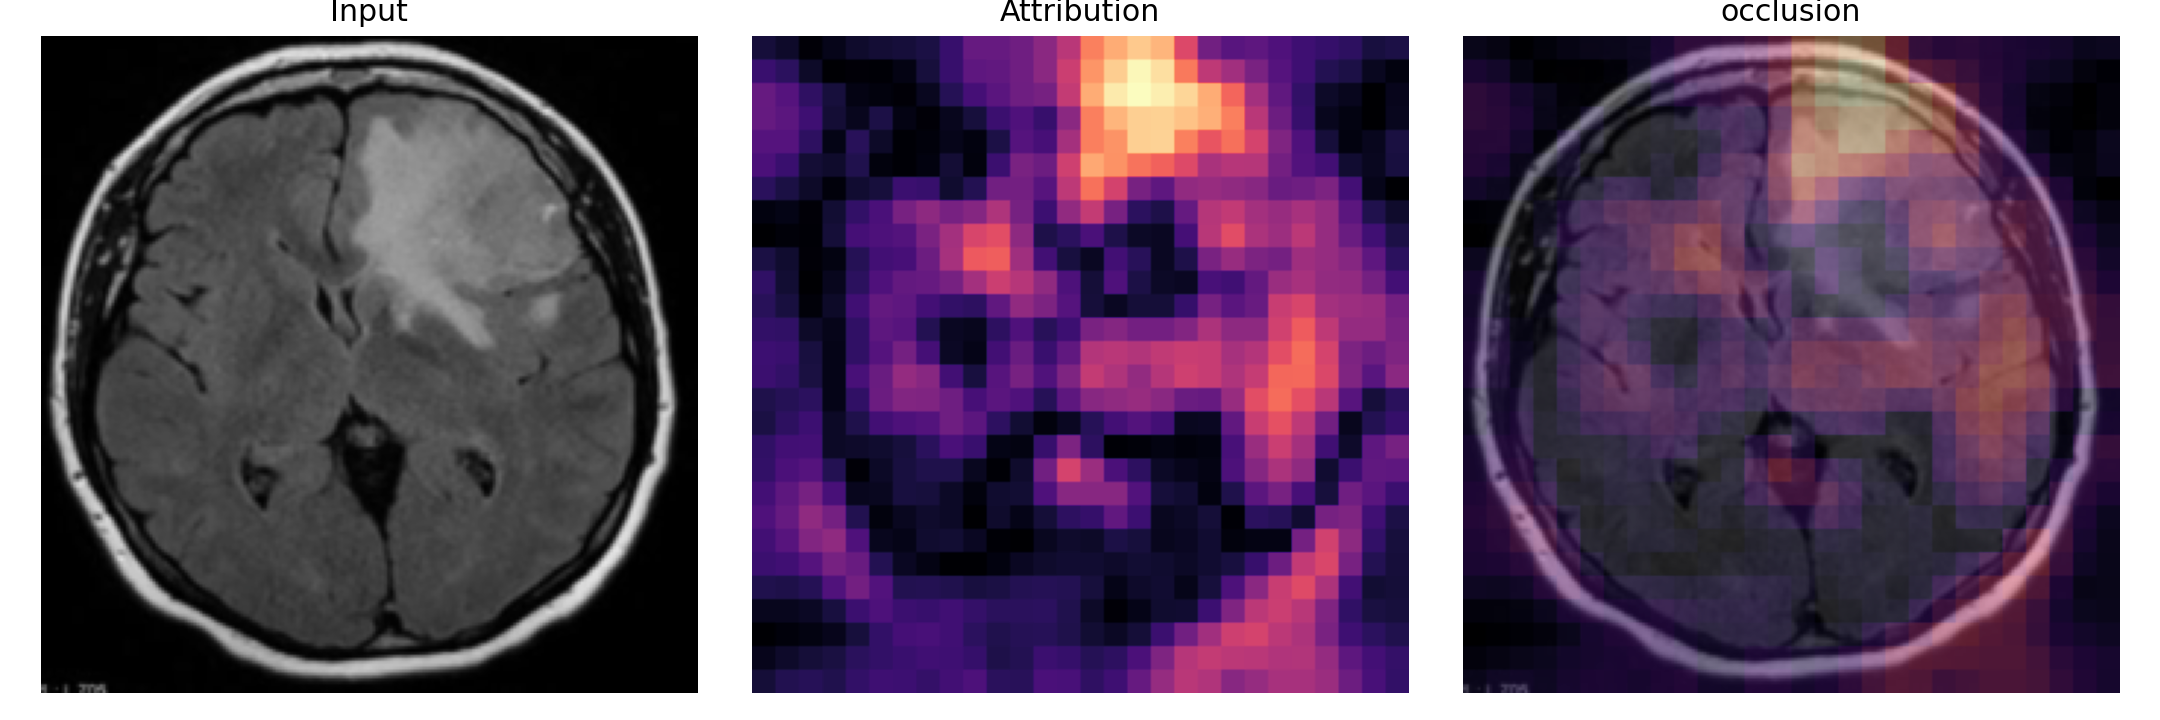
\includegraphics[width=0.46\linewidth]{../results/grenoble_gpu_20260324/xai/yes/Y195/occlusion.png}\hfill
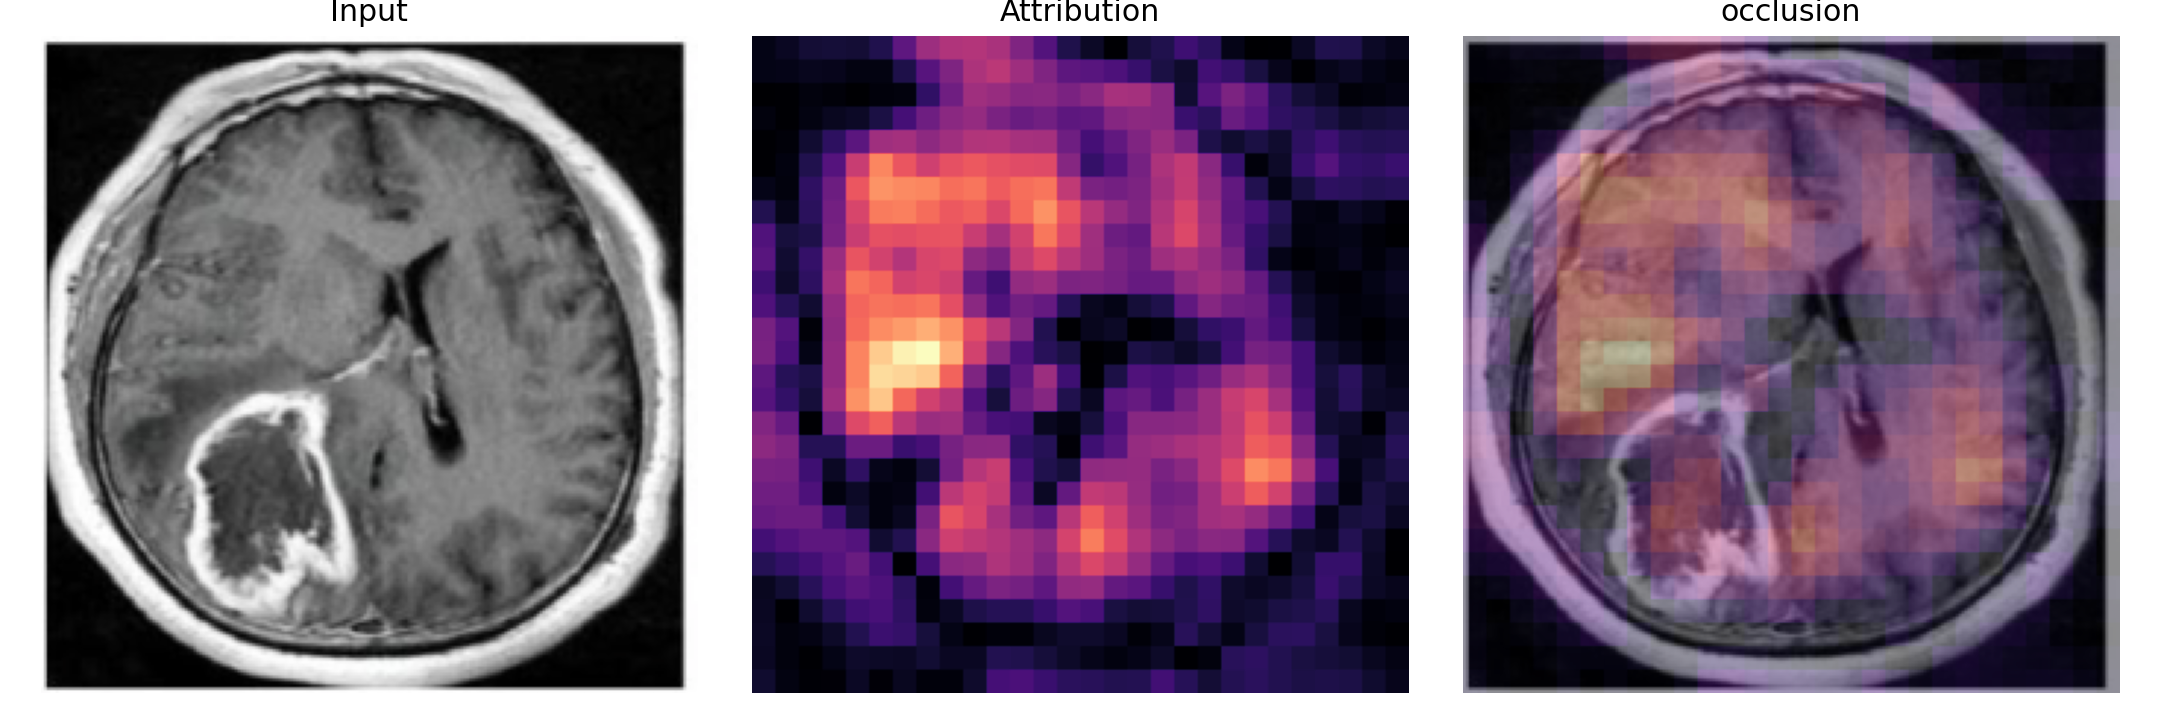
\includegraphics[width=0.46\linewidth]{../results/grenoble_gpu_20260324/xai/yes/Y109/occlusion.png}
\vspace{0.4em}
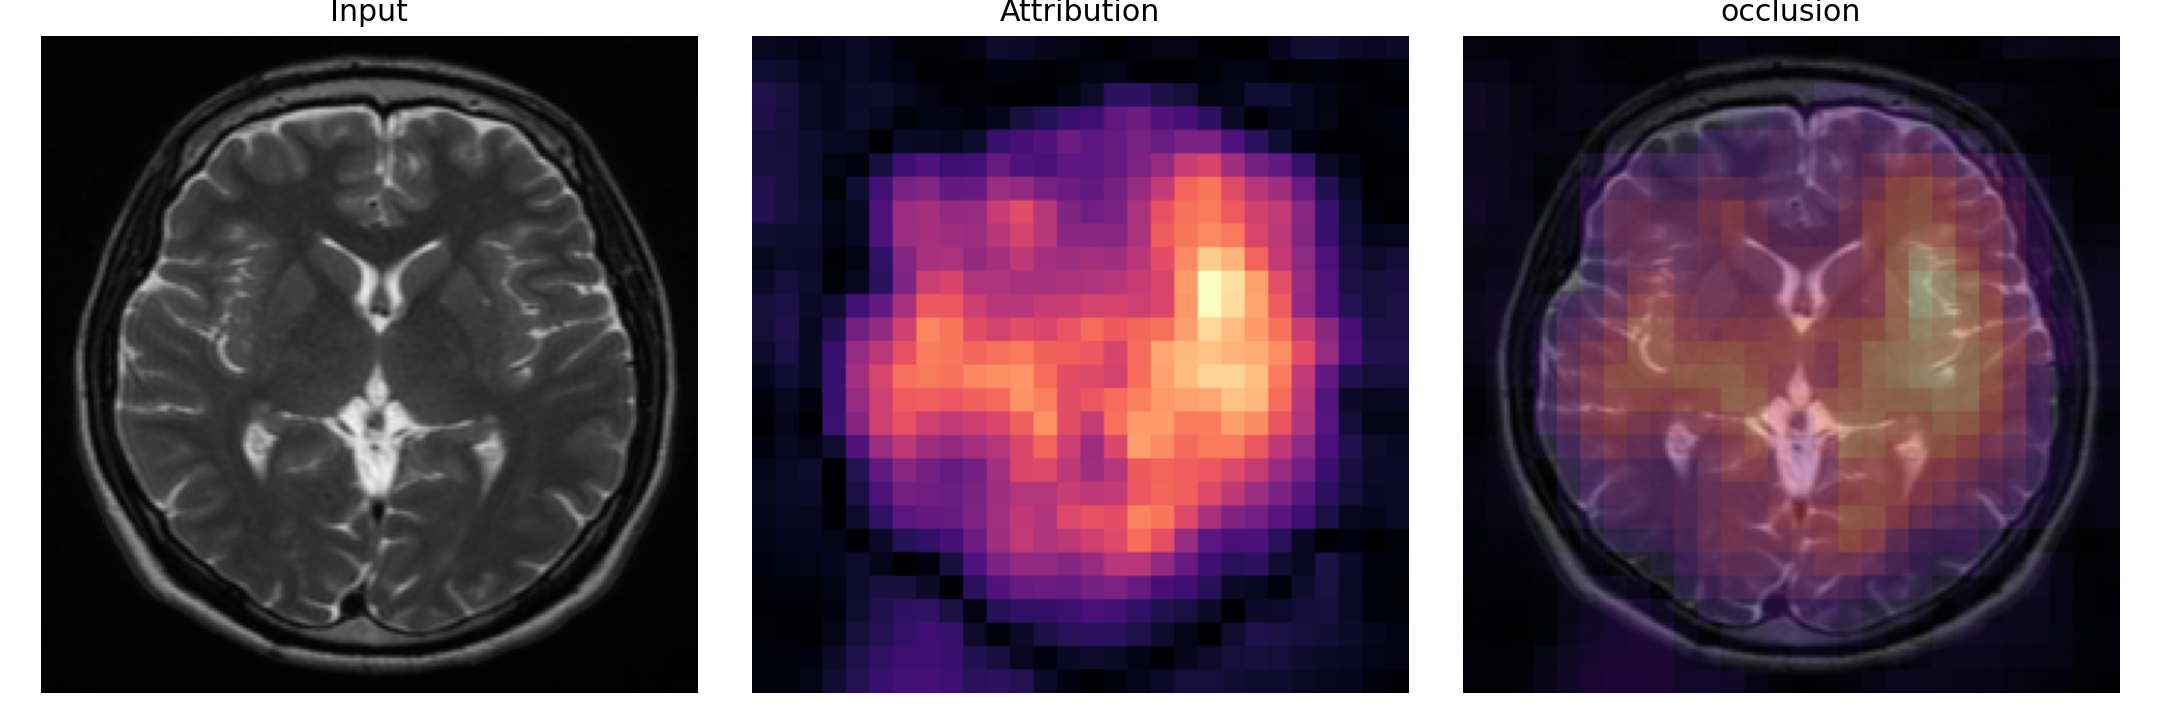
\includegraphics[width=0.46\linewidth]{../results/grenoble_gpu_20260324/xai/no/No22/occlusion.png}\hfill

\includegraphics[width=0.46\linewidth]{\detokenize{../results/grenoble_gpu_20260324/xai/no/4 no/occlusion.png}}
\caption{Même série Brain MRI avec Occlusion. Elle sert à confirmer que les méthodes d'explicabilité donnent une lecture cohérente sur les mêmes cas.}
\end{figure}

\subsection{Pourquoi cette partie reste utile}

La piste Brain MRI n'est pas la piste principale, mais elle garde trois usages
clairs: elle sert de baseline de secours si la partie autoPET pose un problème,
elle fournit un exemple plus simple pour expliquer la XAI à l'équipe, et elle
reste un point de comparaison propre pour le rapport.

\section{Code utile}

Les scripts à connaître vraiment sont résumés ci-dessous.

\begin{tabularx}{\linewidth}{L{5.4cm}Y}
\toprule
\textbf{Script} & \textbf{Rôle concret} \\
\midrule
\texttt{scripts/autopet\_prepare\_fdg.py} & Prépare le sous-ensemble FDG. \\
\texttt{scripts/autopet\_train\_nnunet.py} & Lance l'entraînement \texttt{nnUNet}. \\
\texttt{scripts/autopet\_predict\_nnunet.py} & Produit les métriques de segmentation. \\
\texttt{scripts/autopet\_generate\_xai.py} & Exporte les figures XAI PET/CT. \\
\texttt{scripts/autopet\_export\_results.py} & Crée les snapshots légers pour Git. \\
\texttt{scripts/generate\_xai.py} & Exporte la XAI pour la classification Brain MRI. \\
\bottomrule
\end{tabularx}

Ce sont les scripts qui servent réellement au projet. Le reste est soit de
l'historique, soit du support, soit du résultat d'exploration.

\section{Fichiers à utiliser en priorité}

\begin{tabularx}{\linewidth}{L{5.2cm}Y}
\toprule
\textbf{Fichier ou dossier} & \textbf{Pourquoi il est utile} \\
\midrule
\href{../results/autopet_fdg_full_post_best_dice_50epochs_20260324/segmentation_metrics.json}{Métriques autoPET principales} & C'est la source des chiffres à citer pour la version retenue. \\
\href{../results/autopet_fdg_full_post_best_dice_50epochs_xai_allcases_20260327/xai_analysis_summary.json}{Synthèse XAI autoPET} & Contient les statistiques d'explicabilité sur les 7 cas de revue. \\
\href{../results/autopet_fdg_full_50epochs_variant_comparison_20260324/README.md}{Comparaison autoPET brut vs post-traité} & Résume le compromis entre Dice et faux positifs. \\
\href{../results/grenoble_gpu_20260324/metrics.json}{Métriques Brain MRI} & Donne les scores de la baseline de secours. \\
\href{../results/grenoble_gpu_20260324/xai/}{Figures XAI Brain MRI} & Contient les vrais exemples d'explicabilité à montrer. \\
\bottomrule
\end{tabularx}

\section{Ce qu'on peut ignorer maintenant}

\begin{tabularx}{\linewidth}{L{5.2cm}Y}
\toprule
\textbf{Élément} & \textbf{Pourquoi on l'écarte} \\
\midrule
Le dataset complet à \textasciitilde 400 GB & Il n'apporte pas de gain immédiat pour la rédaction, et il alourdit beaucoup le temps de calcul. \\
Les nouvelles expériences lourdes sans demande explicite & Elles détournent du résultat déjà exploitable. \\
Le multi-traceur / PSMA & Ce n'est pas la cible directe tant que le FDG suffit pour le projet. \\
Les gros artefacts non tracés dans \texttt{results/} & Ils ne sont pas propres à citer ni à partager. \\
\bottomrule
\end{tabularx}

\section{Conclusion}

Le message à garder est simple: on conserve la piste autoPET FDG comme résultat
principal, on garde la classification Brain MRI comme backup, et on s'appuie
maintenant sur les figures et métriques déjà tracées dans Git pour écrire le
rapport ou préparer la présentation. Il n'est pas utile de repartir sur des
expériences lourdes tant que le fond du projet est déjà couvert par ces deux
résultats.

\end{document}
